
\documentclass[11pt]{article}
\usepackage[hmargin=1.5cm,vmargin=1.5cm]{geometry}

\usepackage[affil-it]{authblk}
\usepackage[percent]{overpic}

%\usepackage{ifpdf}
%\ifpdf 
%    \usepackage[pdftex]{graphicx}   % to include graphics
%    \pdfcompresslevel=9 
%    \usepackage[pdftex,     % sets up hyperref to use pdftex driver
%            plainpages=false,   % allows page i and 1 to exist in the same document
%            breaklinks=true,    % link texts can be broken at the end of line
%            colorlinks=true,
%            pdftitle=My Document
%            pdfauthor=My Good Self
%           ]{hyperref} 
%    \usepackage{thumbpdf}
%\else 
%    \usepackage{graphicx}       % to include graphics
%    \usepackage{hyperref}       % to simplify the use of \href
%\fi 

\title{Fast Timing Sexy Title}

\author[1]{D.~Anderson, A.~Apresyan, A.~Bornheim, J.~Duarte, C.~Pena, M.~Spiropulu, S.~Xie}
\author[2]{A.~Ronzhin}
\affil[1]{California Institute of Technology, Pasadena, CA, USA}
\affil[2]{Fermi National Accelerator Laboratory, Batavia, USA}

\date{}

\begin{document}

\maketitle
\abstract{Current and future high energy physics particle colliders are capable
to provide instantaneous luminosities of 10$^{34}$ cm$^{-2}$s$^{-1}$ and above.
The high center of mass energy, large number of simultaneous collision of beam
particles in the experiments and the very high repetition rates of the collision
events pose huge challenges. They result in extremely high particle fluxes,
causing very high occupancies in the particle physics detectors operating at
these machines. We discuss how timing information with a precision of around 10
ps and below can aid the reconstruction of the physics events under such
challenging conditions. 

We present studies and measurements from test beams and GEANT4 simulations for
calorimeter based timing measurements to explore the ultimate timing precision
achievable for high-energy photons. We put particular focus on techniques to
measure the timing with a precision of about 10 ps in association with the
energy of the photon. We present studies with detector prototypes where we
achieve the timing resolution of a few tens of picoseconds in test beam
measurements. Finally, possible applications of precision timing in
future high-energy physics experiments are discussed. }



\section{Introduction}
%shorten the LHC discussion to 1 paragraph
%put the TOF cartoon diagram here and discuss the various aspects affects TOF resolution
% say that we have studied 1,4,5 already, and now we focus on 2 and 3 to complete the story.
% briefly introduce the experiments that we did to understand 2 and 3 ( sampling calo with LYSO cube, shashlik with fibers, shashlik with side readout)

Current and future high energy physics particle colliders are capable to provide
instantaneous luminosities of 10$^{34}$ cm$^{-2}$s$^{-1}$ and above. The high
centre of mass energy, the large number of simultaneous collision of beam
particles in the experiments and the very high repetition rates of the collision
events pose huge challenges. They result in extremely high particle fluxes,
causing very high occupancies in the particle physics detectors operating at
these machines. To reconstruct the physics events, the detectors have to make as
much information as possible available on the final state particles. In addition to
the detailed spatial information of the final state particles, as well as their
momenta and energies, one can make use of the relative time of arrival at a given
location in the detector. The work presented in this document is targeted to
address the challenges posed by the experimental conditions expected for the
high luminosity upgrade of the Large Hadron Collider (HL-LHC) at CERN. 

During the HL-LHC operations the expected instantaneous luminosity is estimated
to be $\mathcal{L}\geq$10$^{34}$~cm$^{-2}$s$^{-1}$, resulting in 140 to 200
simultaneous proton-proton collisions that occur every 25 nsec. The luminous
region inside the detector (the location where the protons collide) will have a
length of a few 10 cm. Due to the size of the proton bunches and the resulting
time it takes for them to pass through each other in the luminous region, the
collisions are spread out in time. During the 2011-2012 operation of LHC this
spread was about 200 ps. For HL-LHC this spread may increase as a consequence of
an advanced beam optics of the interaction region. 

The ATLAS and CMS detectors at the LHC are expected to undergo significant
upgrades and modifications, although the basic geometric layout and size will
remain unchanged. In this work we assume that a detector capable of measuring
the time of arrival of a particle would be located at the outer perimeter of the
tracking device or in the front part of the calorimeter, as for example in the
electromagnetic part of the calorimeter. The typical time scales relevant for
such a setup are: 

\begin{itemize}
  \item Collision time spread within the luminous region is expected to be
        $\sim0.2$--$1.0$ ns.
  \item Typical time of flight of a particle at the speed of light from the
        primary vertex of a proton-proton collision to the location of the
        precision timing device would be in the range of 4~(11)~ns in the barrel
        (endcap) region of the CMS detector.
  \item The size of the shower of electromagnetically interacting particles at
        high energies results in a typical time scale of order 1 ns over which
        the showering process evolved. 
\end{itemize} 

Some of the highest priority goals of the HL-LHC physics program are the
precision measurements of the Higgs boson properties (e.g. in
$H\to\gamma\gamma$), searches (or measurements of properties) of particles
discovered previously in LHC, and studies of the W$_L$W$_L$ scattering. In the
conditions of HL-LHC these physics objectives are challenged by the presence of
high pileup activity, affecting the ability to identify jets that originate from
the vector boson scattering vertex, and degrade the missing transverse energy
resolution. Some fraction of the pileup contamination can be removed through
combination of calorimeter and tracker information. Any calorimeter cluster
originating from a charged hadron can be associated to an extrapolated track as
well and hence to its origin in the collision region. Photons and neutral
hadrons cannot be associated to their production vertex with the tracking
detector. This is where a very precise timing would benefit the event
reconstruction tremendously if a precision of a few 10 ps can be achieved,
corresponding to a few mm resolution at the vertex location~\cite{AdiCalor14}.
To be utilized effectively it seems mandatory that the timing measurement is
very closely linked to the energy measurement, ideally based on the same active
detector element. It is in this context that we study the possibility to measure
the time of arrival of electromagnetic particles with a calorimetric device.

\section{Experimental Setup}
At present we are investigating two options for a calorimeter capable of high
precision timing: a) a dedicated detector based on micro-channel plates (MCP) to
measure shower particles~\cite{MCPFastCaloNIMA}, and b) scintillating crystals
as an active medium to detect the high energy particles and their time of
arrival simultaneously~\cite{AdiCalor14}. This choices are driven by the
potential use case of a precision timing detector for the high luminosity
upgrade of the LHC experiments. For this, the measurement of the time of arrival
of high energy photons with energies of 1 GeV and above is of particular
importance. The study of the dedicated detector was discussed in detail in
Ref.~\cite{MCPFastCaloNIMA}, and in this document we will present a brief
review, while focusing mostly on the option with scintillating crystals. 

Several elements of our experimental setup are shared for studies of the two
options above. In both studies we use MCP-PMT photo-detectors (either Photek 240
or Hamamatsu R3809U-52), and version 4 of the DRS4 evaluation
boards~\cite{DRS4}. We used the Fermilab Test Beam Facility (FTBF), which
provided proton beams from Fermilab's Main Injector accelerator at 120 GeV/c, as
well as secondary electron beams of energies ranging from 4 to 32 GeV/c.
Detectors were located inside of a dark box lined with copper foil for RF
shielding. A 2x2~mm$^2$ scintillator placed inside the box, as shown in
Figure~\ref{fig:SetupLYSO} served as a trigger start signal. For particle
identification we utilized the differential Cherenkov counter located upstream
of our setup.

In the following studies we focus on the extraction of the timing information
from scintillating crystals. We focus our studies on LYSO crystals, which have
an advantage of very high light yield ($\sim 30$K photons/MeV) and radiation
tolerant, and thus are one of the options considered for the CMS upgrade for
HL-LHC. In Figure~\ref{fig:ScintillatorTiming} we present a simplified
experimental setup to illustrate the major contributions to the precision of the
timing measurement with a monolithic, large scintillating crystal. Upon entering
the crystal the photon  needs to convert and start showering to induce
scintillation light in the crystal. We refer to the time scale between entering the crystal
and the first conversion as $t_C$. The
scintillation process is usually described by two time constants: the rise time
of the scintillation light and its typical decay constant. The rise time of the
scintillation light signal from LYSO crystals has been measured to on the order
of 75 ps~\cite{LYSOrisetime}. The decay time constant for LYSO is on the order
of 40 ns. For high energy particles in the multi GeV range the shower even for
electromagnetic particles will extend over several centimeters, taking on the
order of a nanosecond. With our current experimental setup we cannot
de-convolute the time structure of the scintillation process and the propagation
of the shower through the crystal. We denote the related characteristic time
constant with $t_S$. 

\begin{figure}[h] \centering
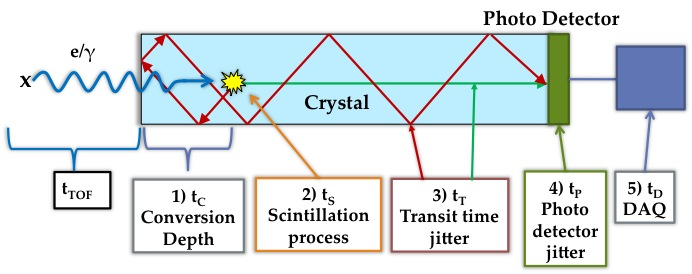
\includegraphics[width=0.85\textwidth]{figs/ScintillatorTiming} \caption{Factors
influencing the precision of the timing measurement with a monolithic, large
scintillating crystal. The incident particle impinges on the crystal face from
the left. Characteristic times of various factors are defined in the colored
boxes and in the text.}
\label{fig:ScintillatorTiming}
\end{figure}

The scintillation light produced needs to be detected. Typically this is done
with one or several photo detectors attached to the scintillator. The time $t_T$
it takes the scintillation photons to travel through the crystal may vary
substantially due to the isotropic angular distribution of the scintillation
light and the possible internal reflection of the light inside the crystal
before eventually reaching the photo detector. Finally, the photo detector and
its readout system have characteristic time constants $t_P$ and $t_D$ which will
affect the precision of the measurement as well.

In this study we focus on studying the effects of the shower development,
scintillation light emission and light propagation inside the crystal. Since the
photodetectors and readout system are shared with the experiment described
in~\cite{MCPFastCaloNIMA}, the chararacteristic times $t_P$ and $t_D$ are shared
between these two measurements. In our measurements in
Ref.~\cite{MCPFastCaloNIMA} we found the time-of-flight resolution between the
Photek 240 detectors to be $\sim 15$psec~\footnote{Here and in the following we
refer the standard deviation of the Gaussian fit as the ``resolution''}.
Assuming that the resolution of both Photek 240 is the same, one can derive the
time resolution of a Photek 240 to be $15/\sqrt{2}\approx$11 ps. The electronic
resolution of the DRS4 board was found to be $5-7$ psec. 

\begin{figure}[h] \centering
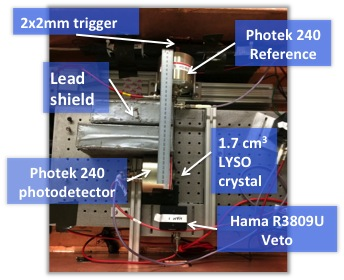
\includegraphics[width=0.5\textwidth]{figs/SetupLYSO} 
\caption{Experimental
setup for the test beam measurements. Inside a light tight box, shielded against
environmental noise, a LYSO crystal is mounted on one of the Photek 240
detectors. In all measurements the 2x2 mm$^2$ scintillator was used for
triggering. The reference Photek 240 is placed right after the trigger, and a
Hamamatsu R3809 MCP is placed behind the crystal as a Veto detector. Lead bricks
are placed upstream of the Photek 240 that reads out the crystal, to shield the detector from 
direct hits on MCP-PMT detector from beam particles.} 
\label{fig:SetupLYSO}
\end{figure}


In all results presented here which invoke the MCP based reference detector
measurement we did not unfold its contribution to the final result. In the
initial studies presented here we focus on measurements which allow to quantify
the contribution of the showering process in the crystals, the scintillation
light emission and the light propagation inside the crystal. These contributions
will dependent on the type of scintillator used, its size and its surface
properties. Future experiments will be carried out to study all these factors in
detail.

\section{Event Selection and Analysis}
To assign a time stamp for each signal
pulse, we use different procedures for the reference detector and for the one
with LYSO crystal, since their pulses have different shapes. The pulse from the
reference detector is a very sharp and symmetric around its maximum amplitude,
as shown in Figure~\ref{fig:PulseShapes}. Therefore, for the reference detector
the assignment of a time stamp is the following. We first determine the time
position of the pulse peak. A Gaussian function is fitted to the pulse maximum
using three points before the maximum of the pulse peak and four points after
the maximum. The mean value of the Gaussian fitted function was used as the time
stamp for each pulse. A time stamp for the scintillation light is assigned using
constant fraction fit on the rising edge. We perform a fit with a linear
function between the points at 20\% and 70\% of the maximum of the pulse peak,
and the time stamp is assigned as the midpoint of the fitted function. Examples of fits performed to assign a time stamp from each pulse are shown in Figure~\ref{fig:PulseFits}.

\begin{figure}[h] \centering
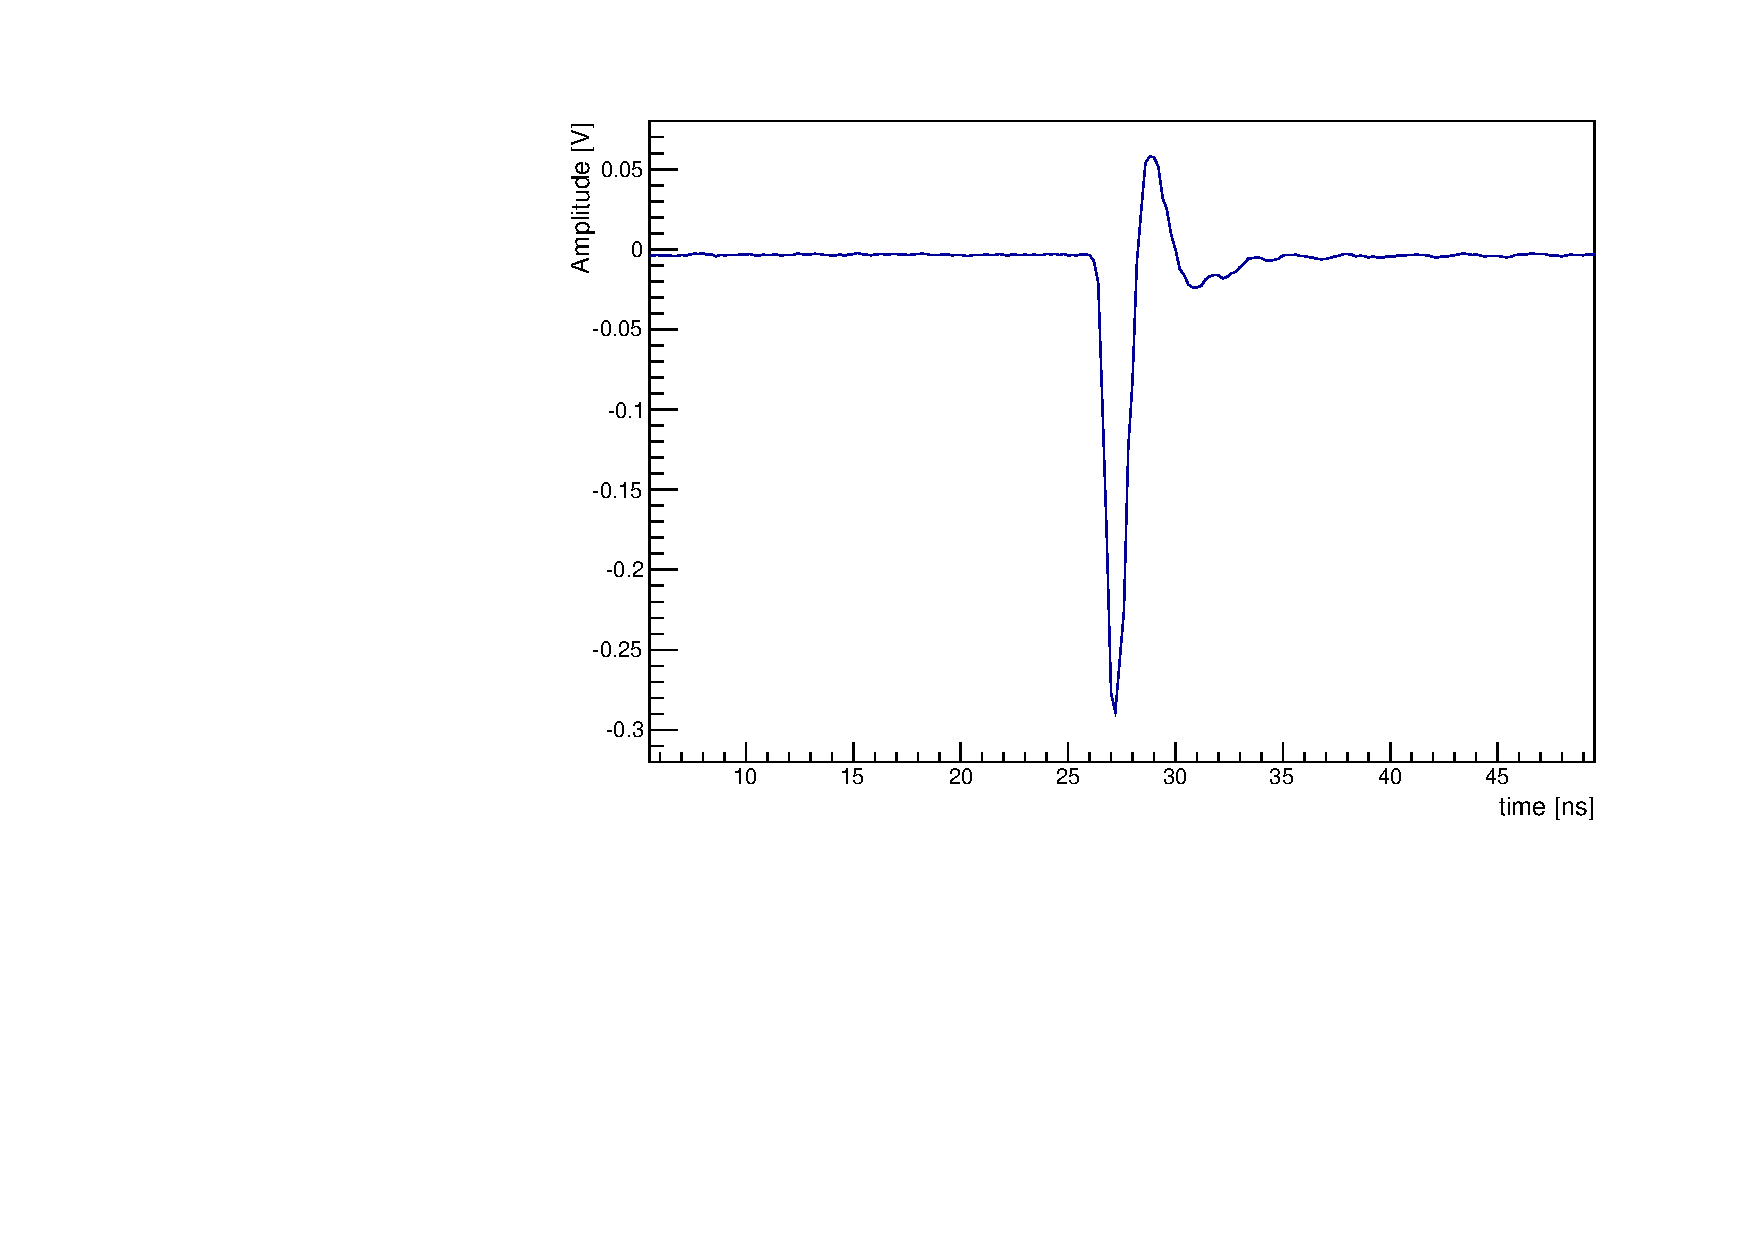
\includegraphics[width=0.45\textwidth]{figs/RefPulse} 
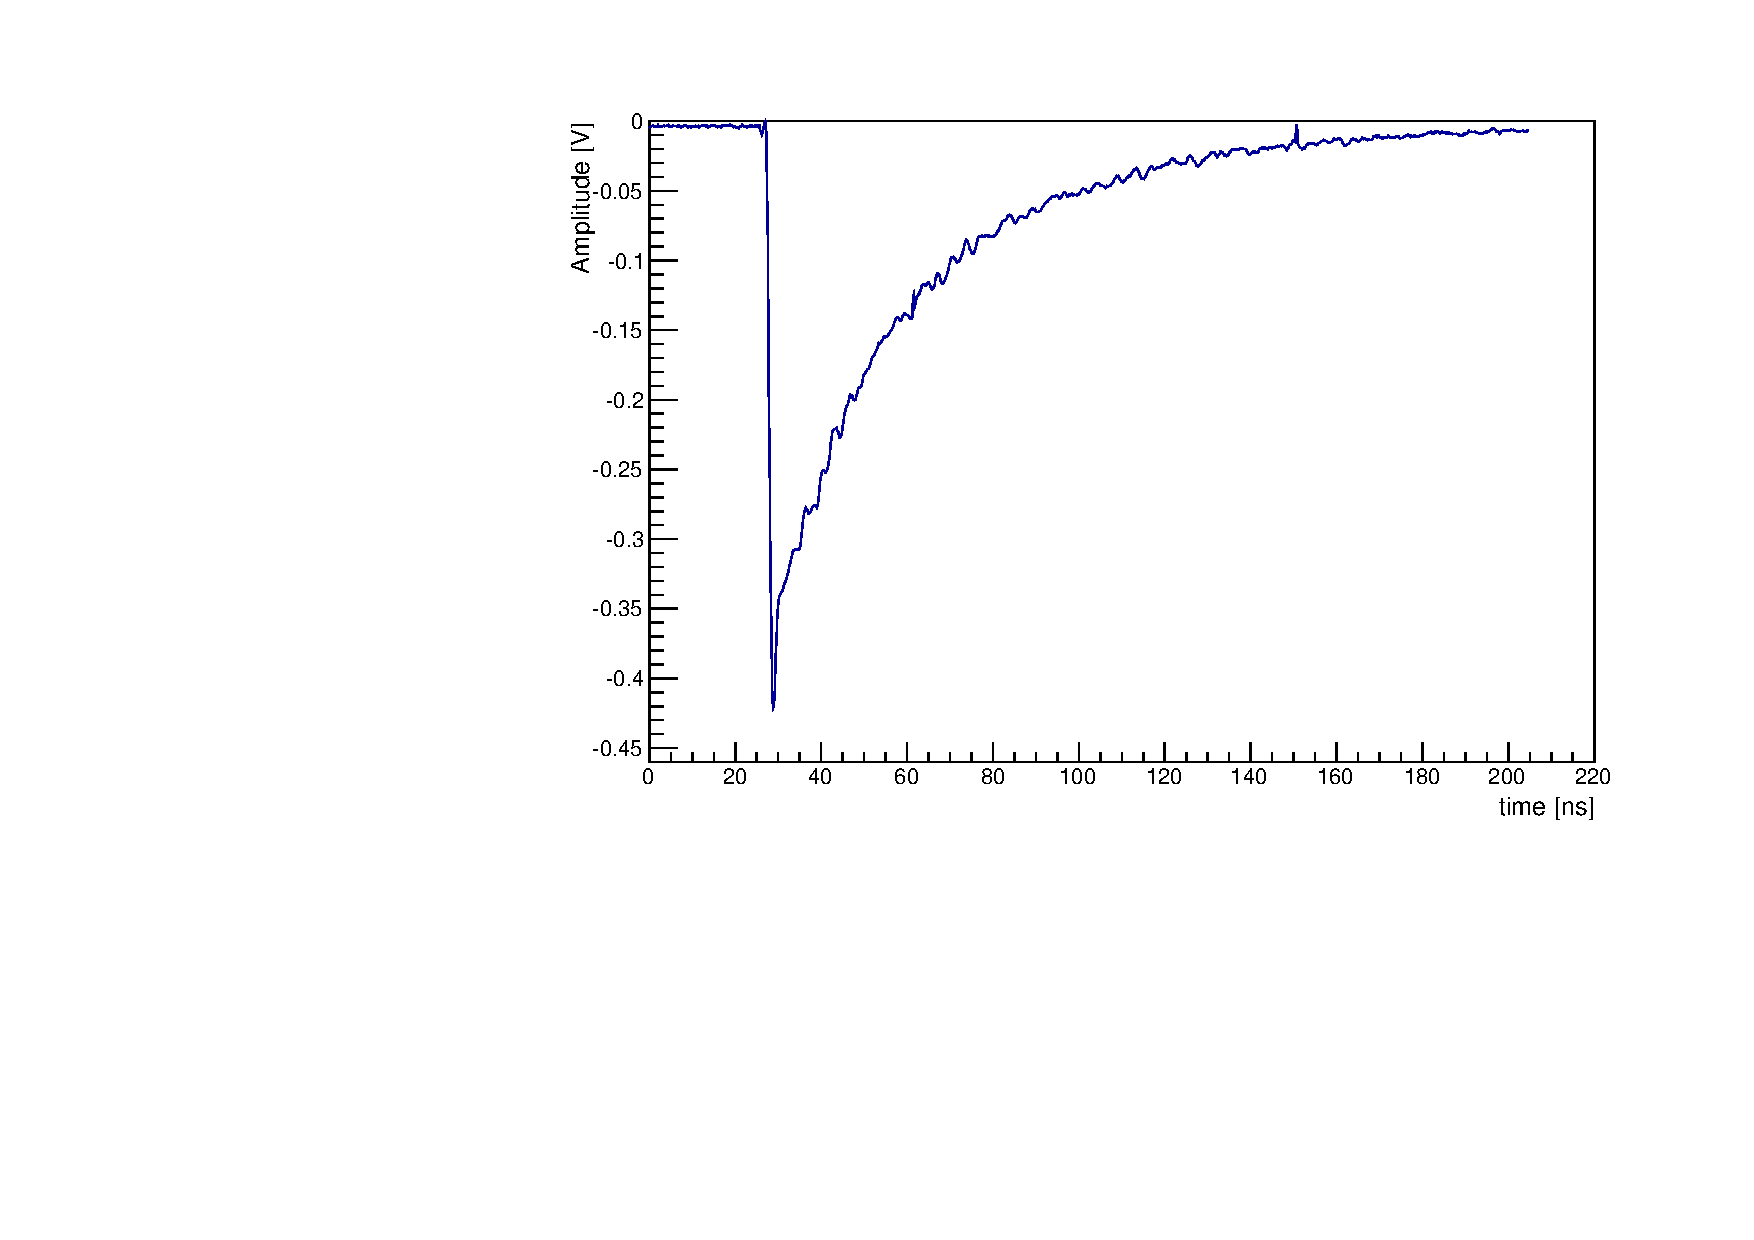
\includegraphics[width=0.45\textwidth]{figs/ScintPulse} 
\caption{Sample pulses as digitized by the DRS4 board. (Left) is a  pulse from the reference Photek 240, and (right) is a  pulse from 1.7 cm$^3$ LYSO crystal, from an 8 GeV electron run.} 
\label{fig:PulseShapes}
\end{figure}

Event selection and pulse cleaning procedure was used to eliminate abnormal
pulses in the readout. Large signals above 500 mV were also rejected because
they saturated the DRS4 inputs. Pulses with an irregular peak profile were
rejected, as well as pulses which experienced a sudden reversal of polarity that
is occasionally observed with our readout. We selected the pulses with amplitude
larger than 20 mV for future analysis. Events containing more than one pulse
within our readout window of 200 ns were not used. 

\begin{figure}[h] \centering
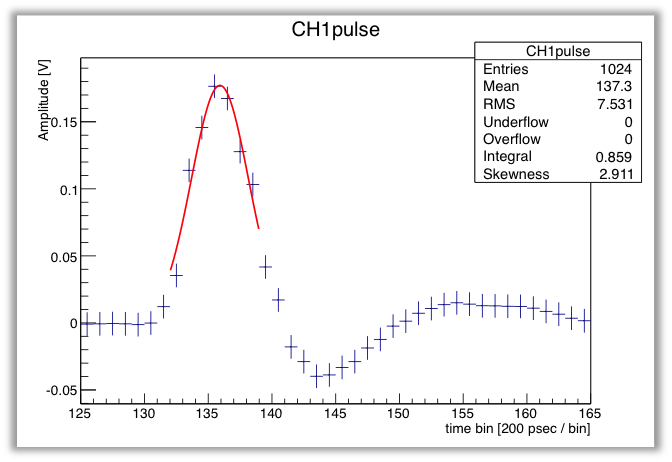
\includegraphics[width=0.45\textwidth]{figs/RefPulseFit} 
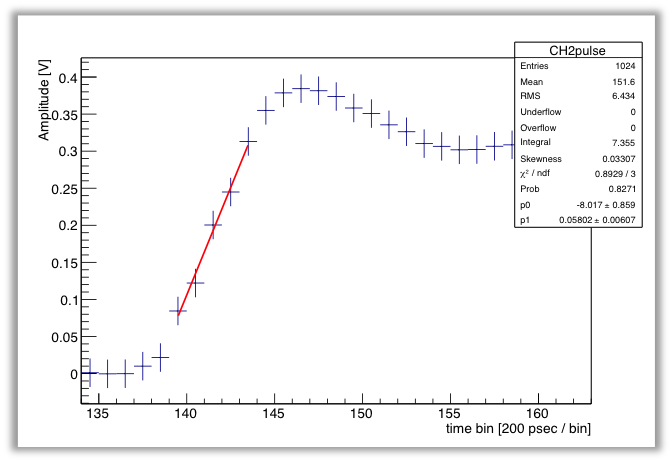
\includegraphics[width=0.45\textwidth]{figs/ScintPulseFit} 
\caption{Sample fits to assign a time stamp to the each pulse. (Left) is a  pulse from the reference Photek 240, and (right) is a  pulse from 1.7 cm$^3$ LYSO crystal, from an 8 GeV electron run.} 
\label{fig:PulseFits}
\end{figure}


\section{Time of Flight in LYSO Crystal-based Calorimeters}

As we discussed in the introduction, this article describes studies
focused on the characterization of two of the five main aspects
driving the time of flight resolution: scintillation and 
optical transport. Stochastic processes in the scintillation
mechanism and the randomization of the optical paths for the 
scintillation light to reach the location of the photodetector 
affect both the speed of the signal formation
as well as the time jitter. We characterize the impact of
these two effects on the time of flight resolution using
two independent experimental setups which isolates the
two components. To study the effect of scintillation
we perform time of flight resolution measurements
for electron beams using a sampling calorimeter composed of a 
$(1.7\mathrm{ cm})^{3}$ LYSO cube as the active 
scintillating element behind about 4 radiation lengths of lead. 
The effect of optical transport is studied by measuring
the time of flight resolution using a shashlik 
calorimeter composed of alternating layers of tungsten
and LYSO, with scintillation light signal extracted
through wavelength shifting fibers as well as 
through direct optical coupling to the edges of a few
LYSO layers. 


\subsection{Studies of Time Jitter from Scintillation}

We study the impact of the scintillation mechanism in LYSO
on the time of flight resolution using a simple 
sampling calorimeter composed of a layer of
lead, about $4.5$ radiation lengths in thickness, acting
as a radiator and a LYSO crystal cube with linear dimensions 
of $1.7$~cm. The LYSO crystal is wrapped in Tyvek and  
coupled with optical grease to a Hamamatsu R3809 MCP-PMT
which is used to extract the scintillation photon signal. 
A Photek 240 MCP is placed upstream of the calorimeter and 
is used to measure the reference time. A schematic diagram
and a photograph of the experimental setup
is shown in Figure~\ref{fig:LYSOSamplingCaloSetup}. 
The contribution of optical transit effects on the 
time of flight resolution is minimized as the linear
dimensions of the cube is relatively small.

\begin{figure}[h] \centering
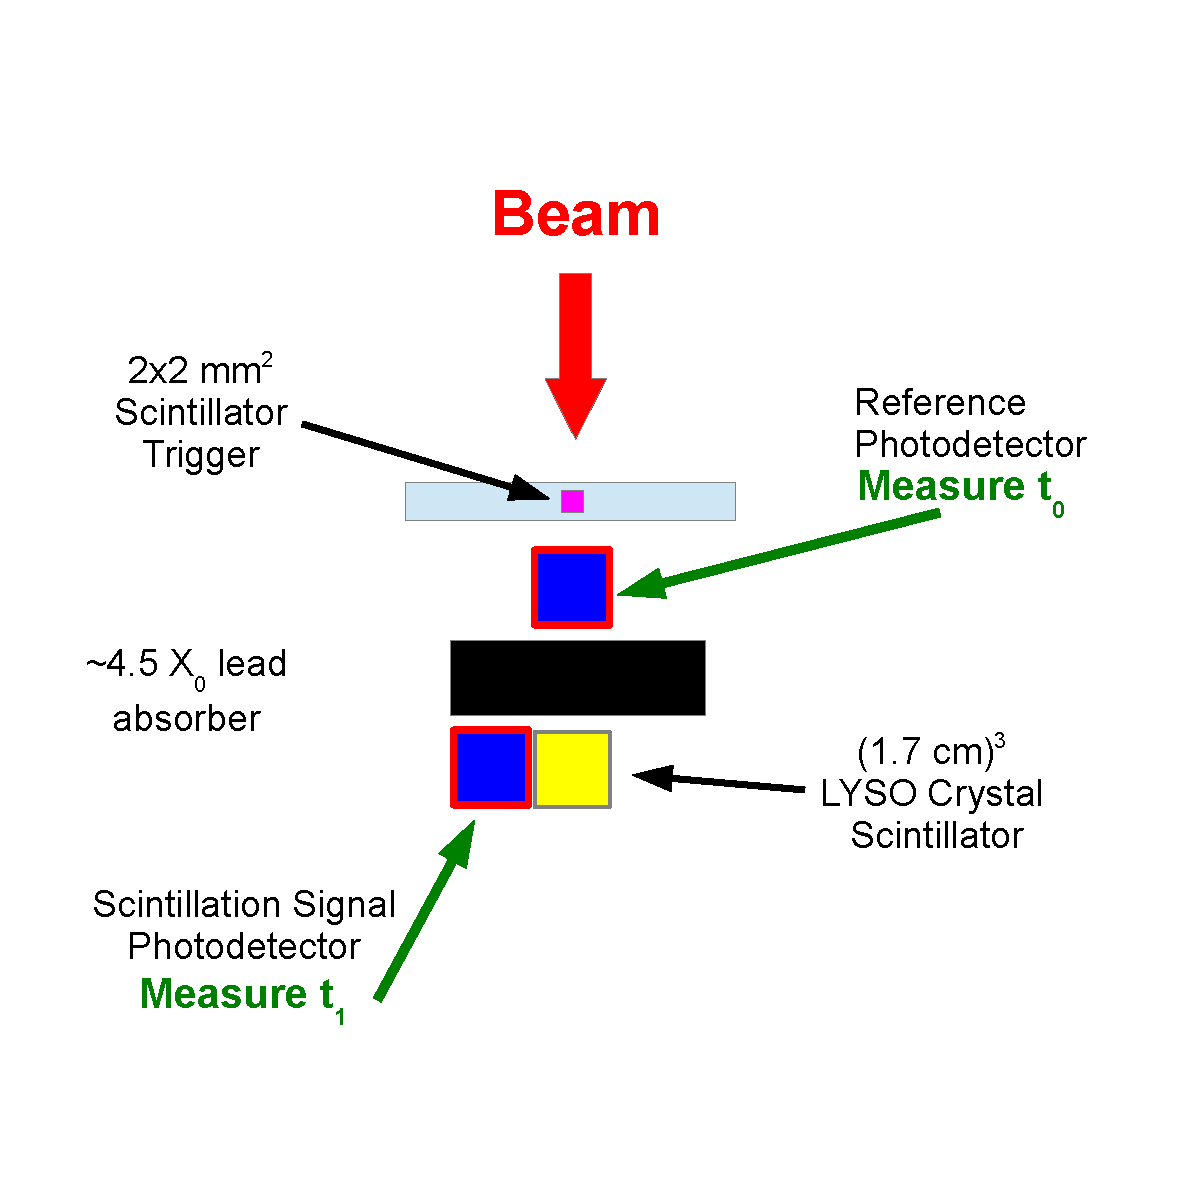
\includegraphics[width=0.45\textwidth]{figs/LYSOSamplingCaloSetupSchematic} 
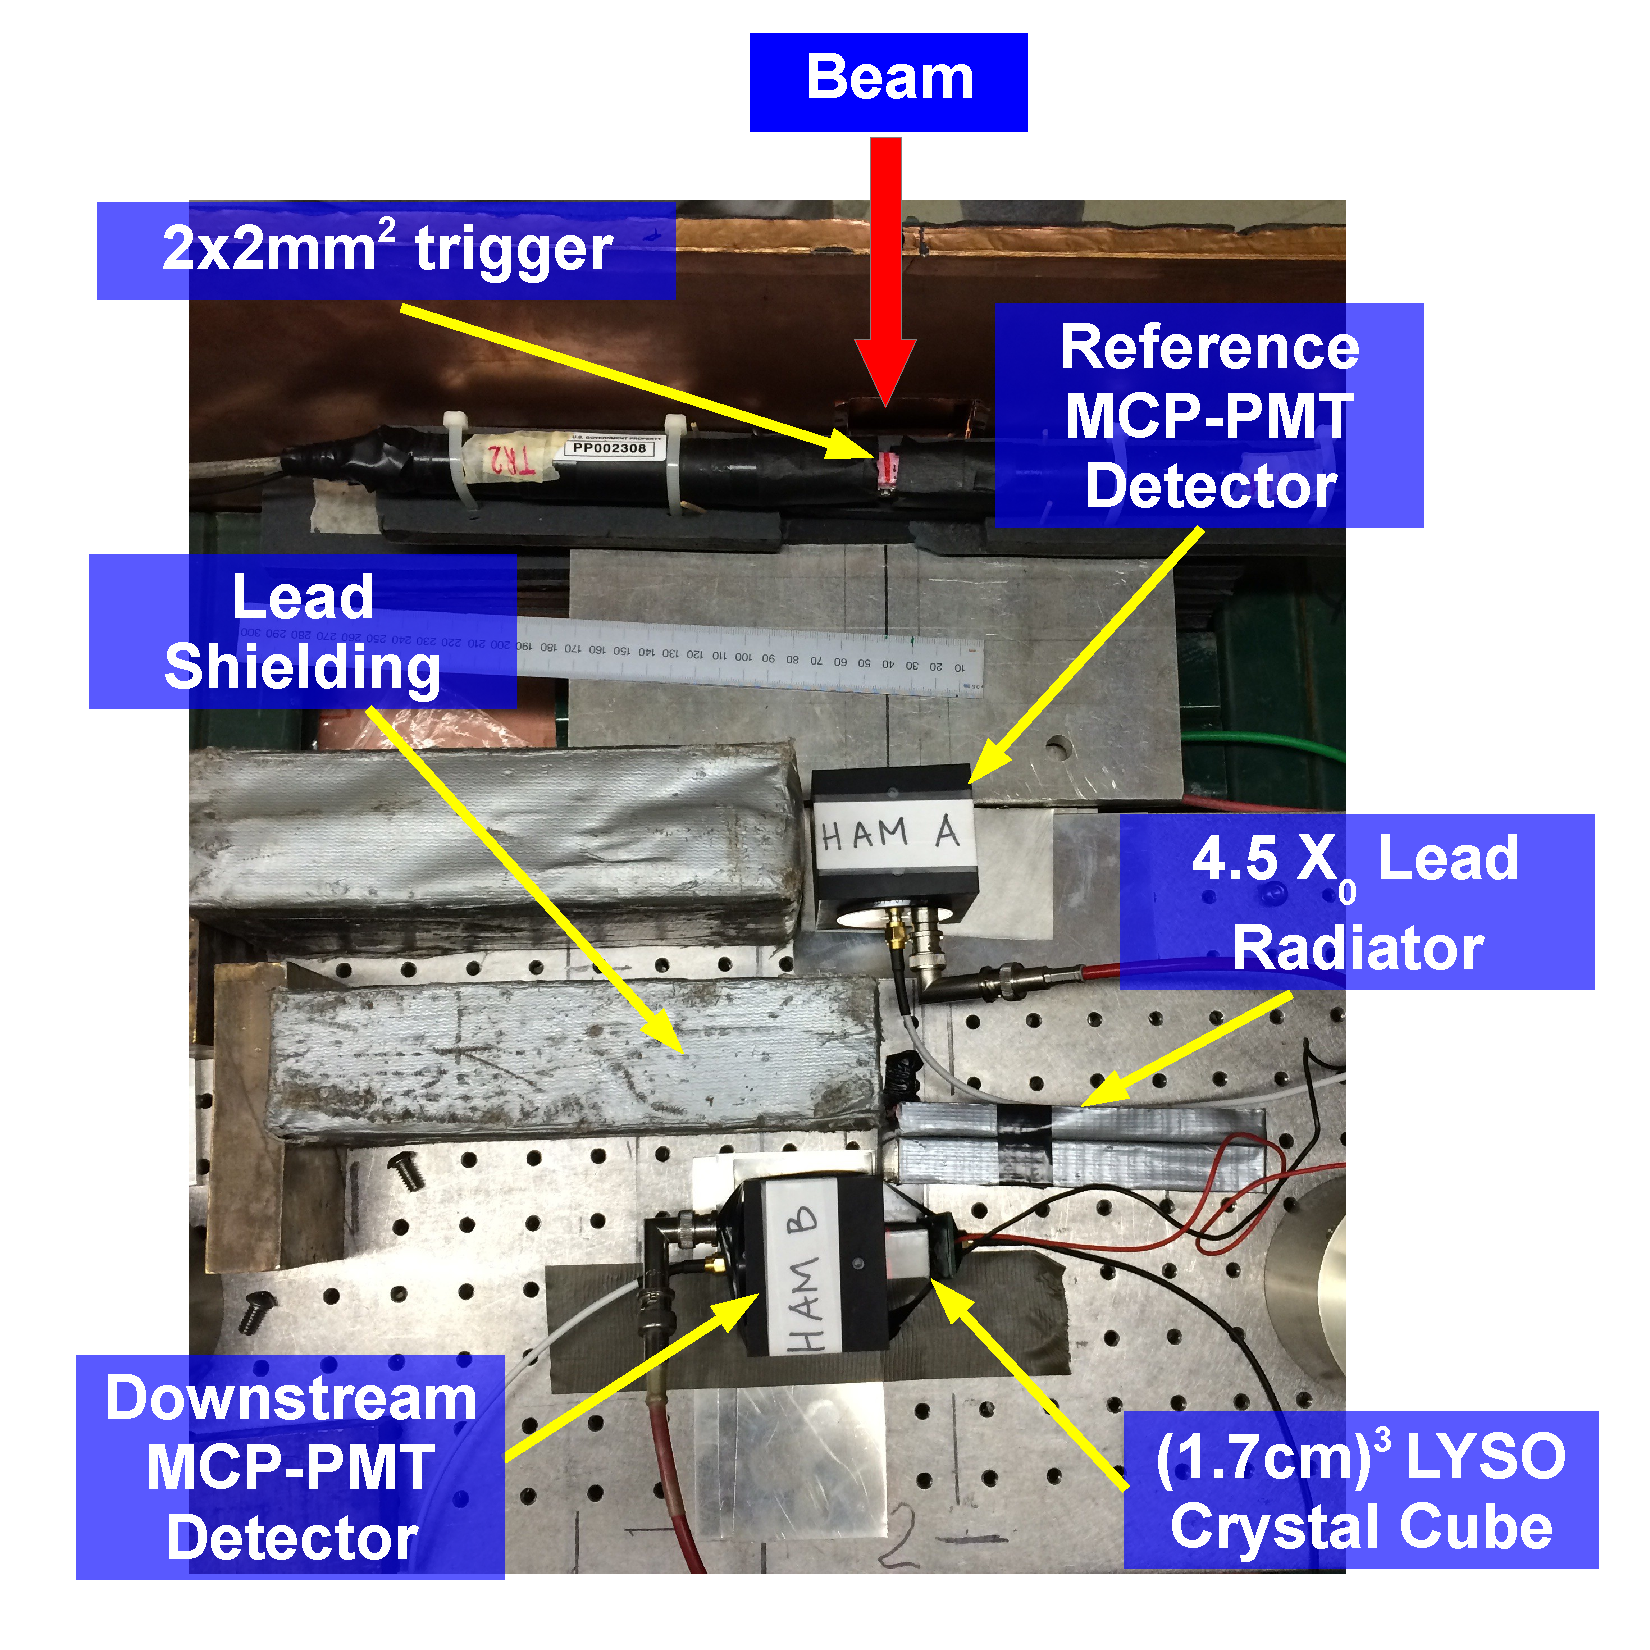
\includegraphics[width=0.45\textwidth]{figs/LYSOSamplingCaloSetupPhoto} 
\caption{ A schematic diagram of the experimental setup for the
time of flight measurement using the LYSO sampling calorimeter
is shown, along with a photograph of the experimental setup. } 
\label{fig:LYSOSamplingCaloSetup}
\end{figure}

A plastic scintillator, approximately $2$~mm by $2$~mm in cross sectional area
and placed upstream of the reference time detector, is used to trigger
the DAQ readout on the DRS waveform digitizer and ensures that any
time of flight measurement is constrained to within a $2$~mm region,
which limits the time jitter due to the geometry to about $12$~ps. 
Electron events were identified by requiring a signal with amplitude
larger than $10$~mV in the Cherenkov counter.
Finally, large lead bricks are placed upstream of the Hamamatsu
R3809 MCP-PMT but out of the beam to provide shielding of the photodetector
from stray particles produced from events where an electromagnetic shower
occurs elsewhere upstream of the lead radiator. Such stray shower
events yield very fast signals which can significantly contaminate the
scintillation signal if uncontrolled. Using the identical
experimental setup but without the LYSO active element in place,
we found that stray shower type events yield less than $10\%$ contamination
and gives a negligible effect on the scintillation signal. The same calorimeter
setup using the Photek 240 MCP in place of the Hamamatsu R3809 MCP-PMT,
which has an active area about $10$ times larger, was found to yield 
more than $80\%$ contamination and thus did not result in a proper
measurements of the scintillation signal.

Despite the thickness of the LYSO active element layer being relatively
small and therefore only capturing a fraction of the total energy
of the electron, the location of the active element is relatively close to the
shower maximum for electromagnetic showers, and yields
a reasonable energy measurement. In Figure~\ref{fig:LYSOCubeEnergy32GeV}
we show the distribution of the pulse integral for events
measured by this sampling calorimeter produced with a
$32$~GeV electron beam, and find a resolution of about $20\%$.


\begin{figure}[h] \centering
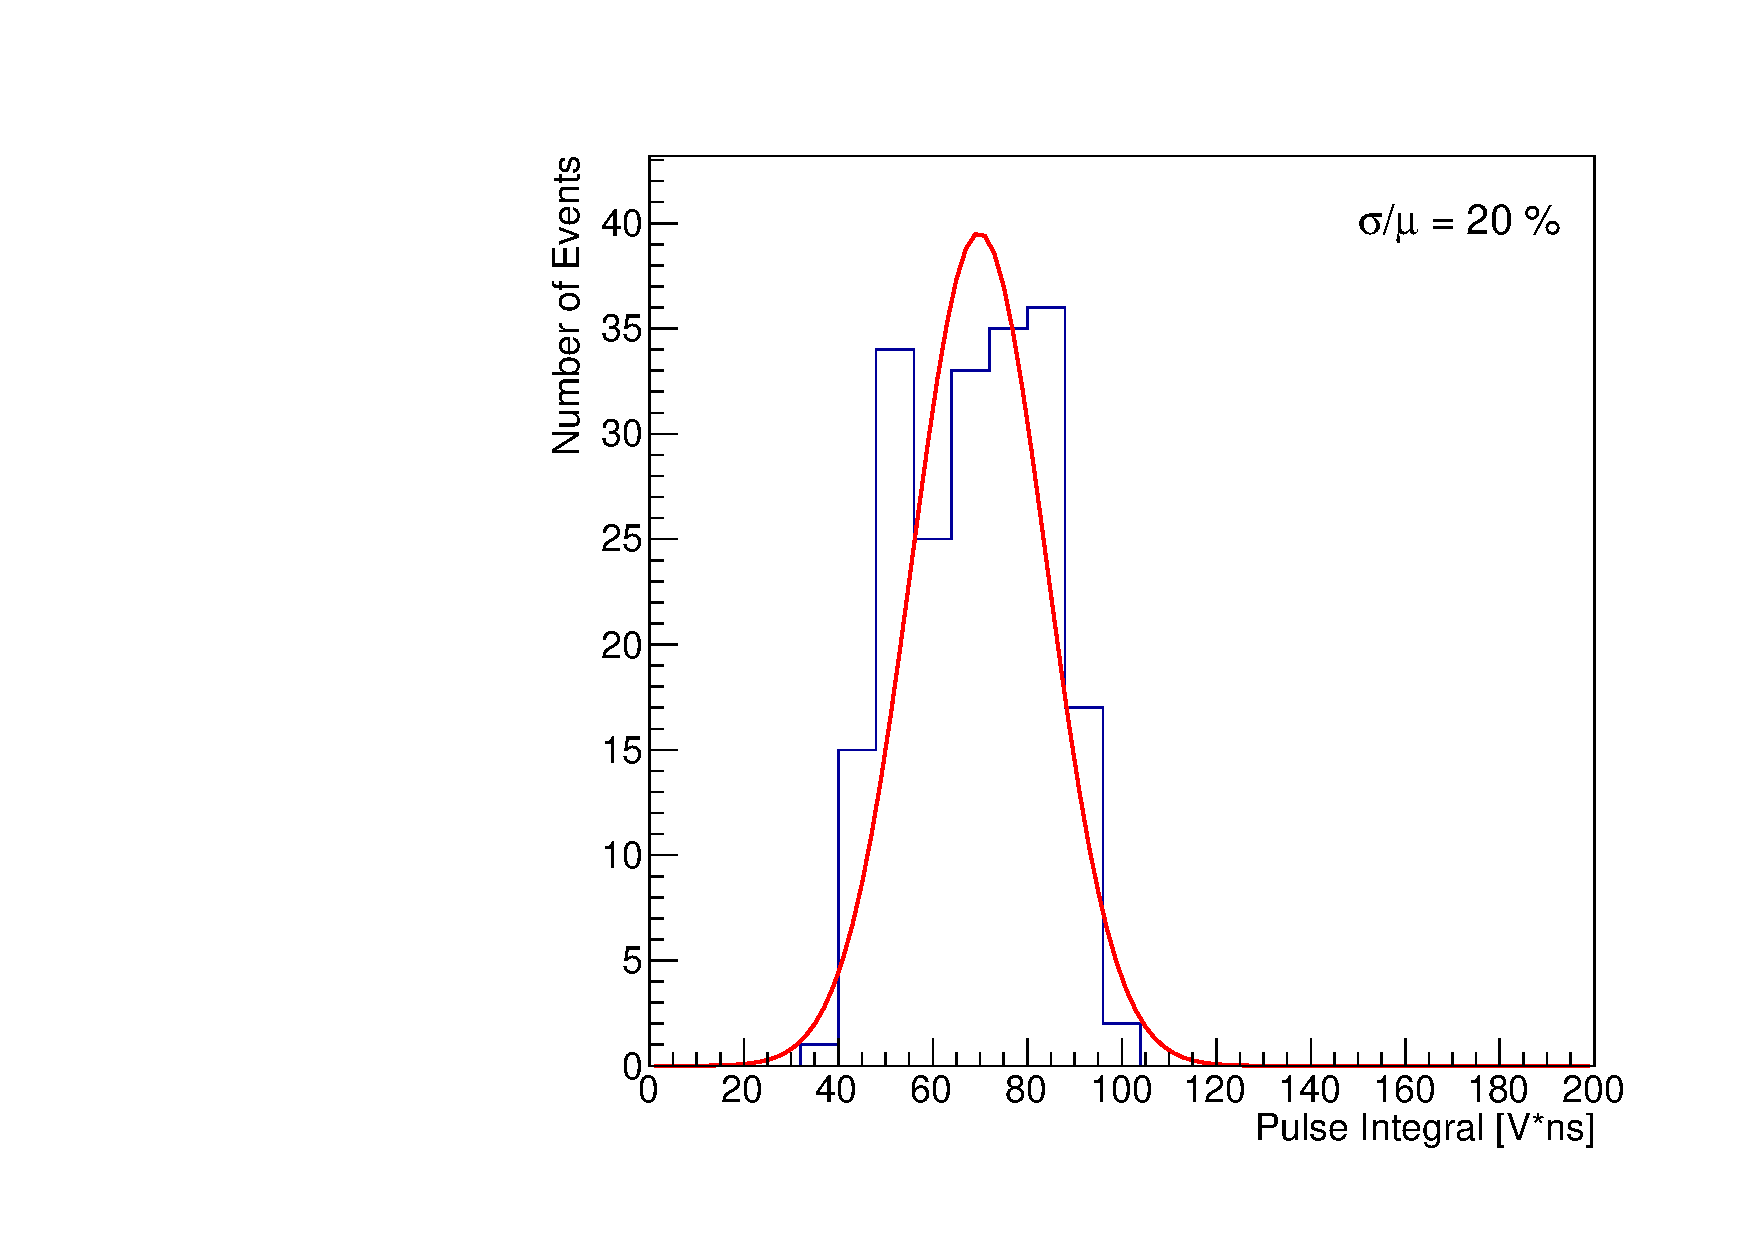
\includegraphics[width=0.45\textwidth]{figs/TOF_Electron_LYSOCube_32GeV_energy} 
\caption{ Histogram of the pulse integral for events recorded using
the LYSO cube sampling calorimeter for a $32$~GeV electron beam. } 
\label{fig:LYSOCubeEnergy32GeV}
\end{figure}

The time of flight measurement was performed using the LYSO sampling calorimeter
for electron beams with energies varying from $4$~GeV to $32$~GeV. The 
measured time of flight distributions are shown in Figure~\ref{fig:LYSOCubeTOF}.
We achieve the best time of flight resolution of $34$~ps for electrons
with beam energy of $32$~GeV.

\begin{figure}[h] \centering
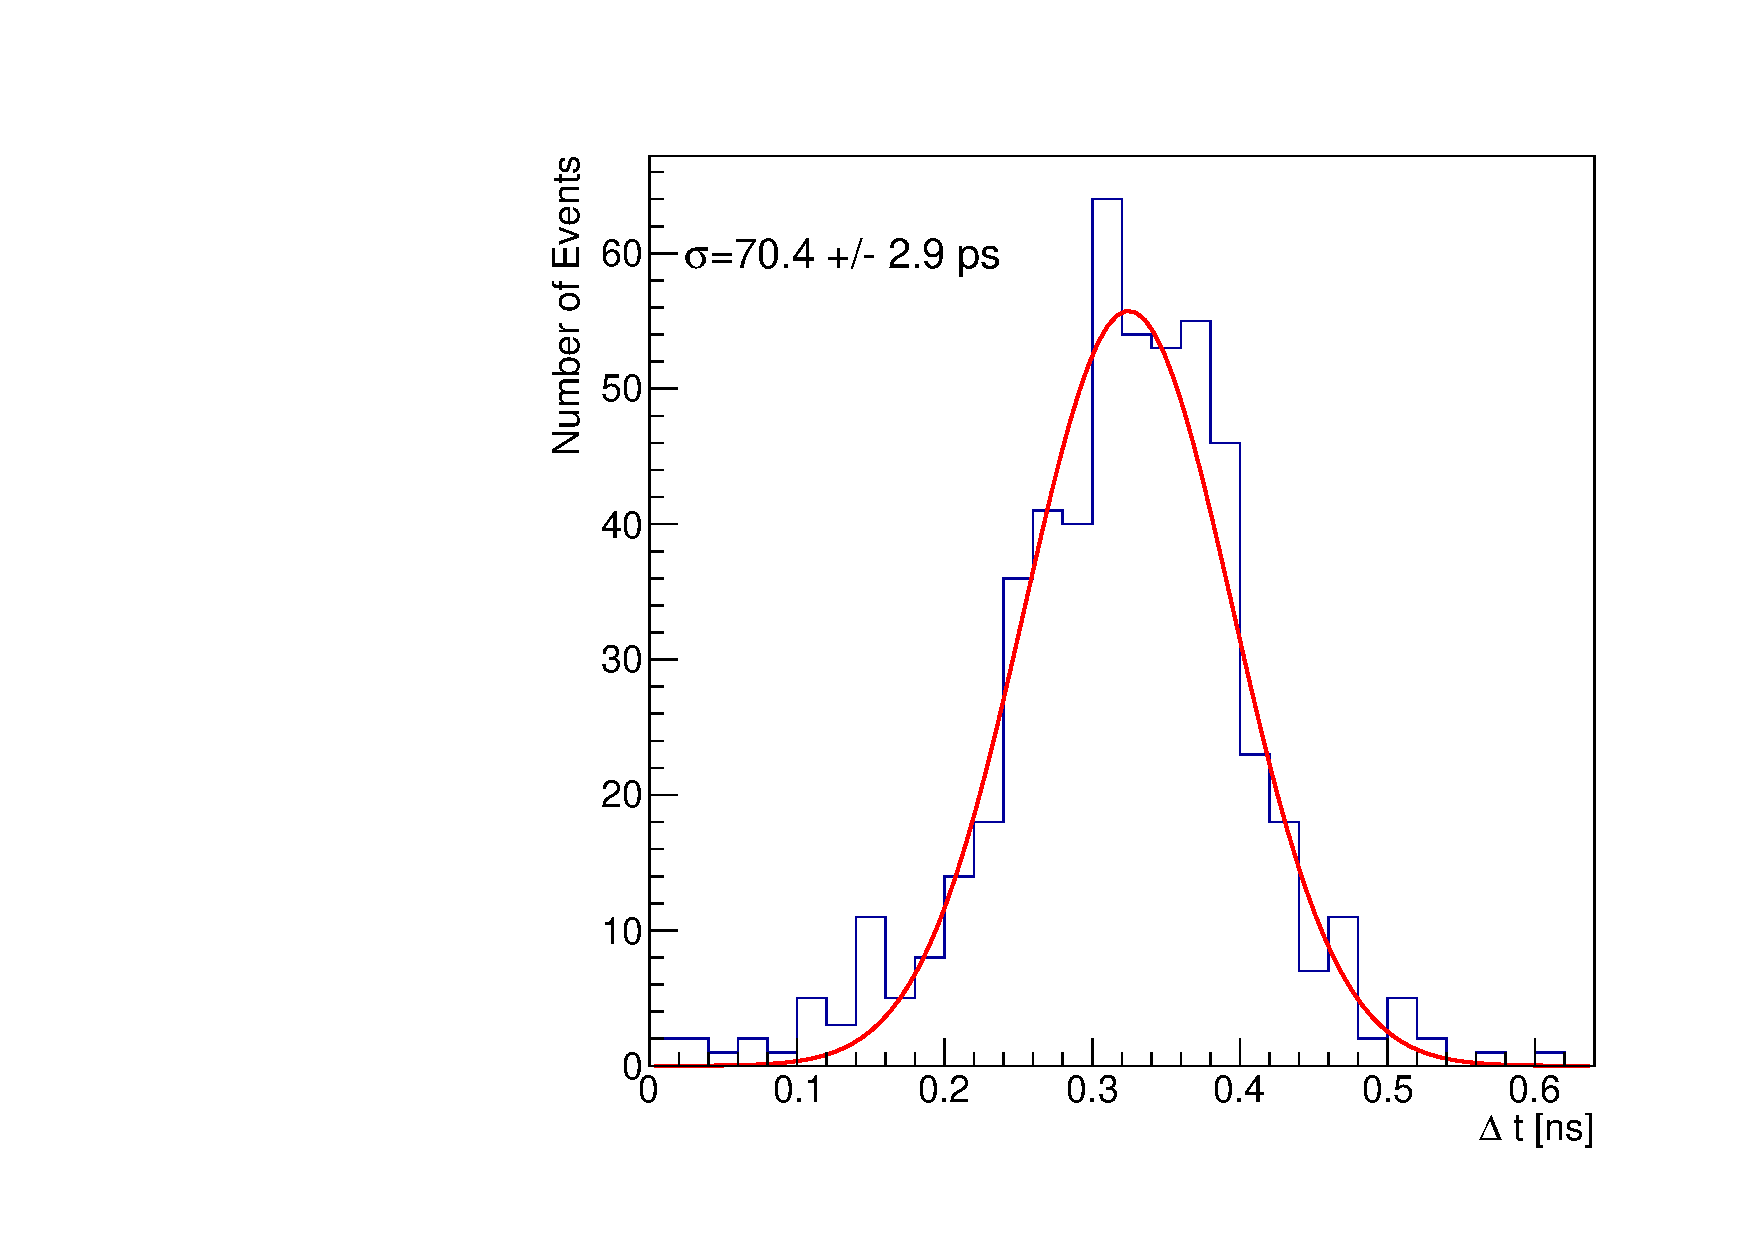
\includegraphics[width=0.45\textwidth]{figs/TOF_Electron_LYSOCube_4GeV} 
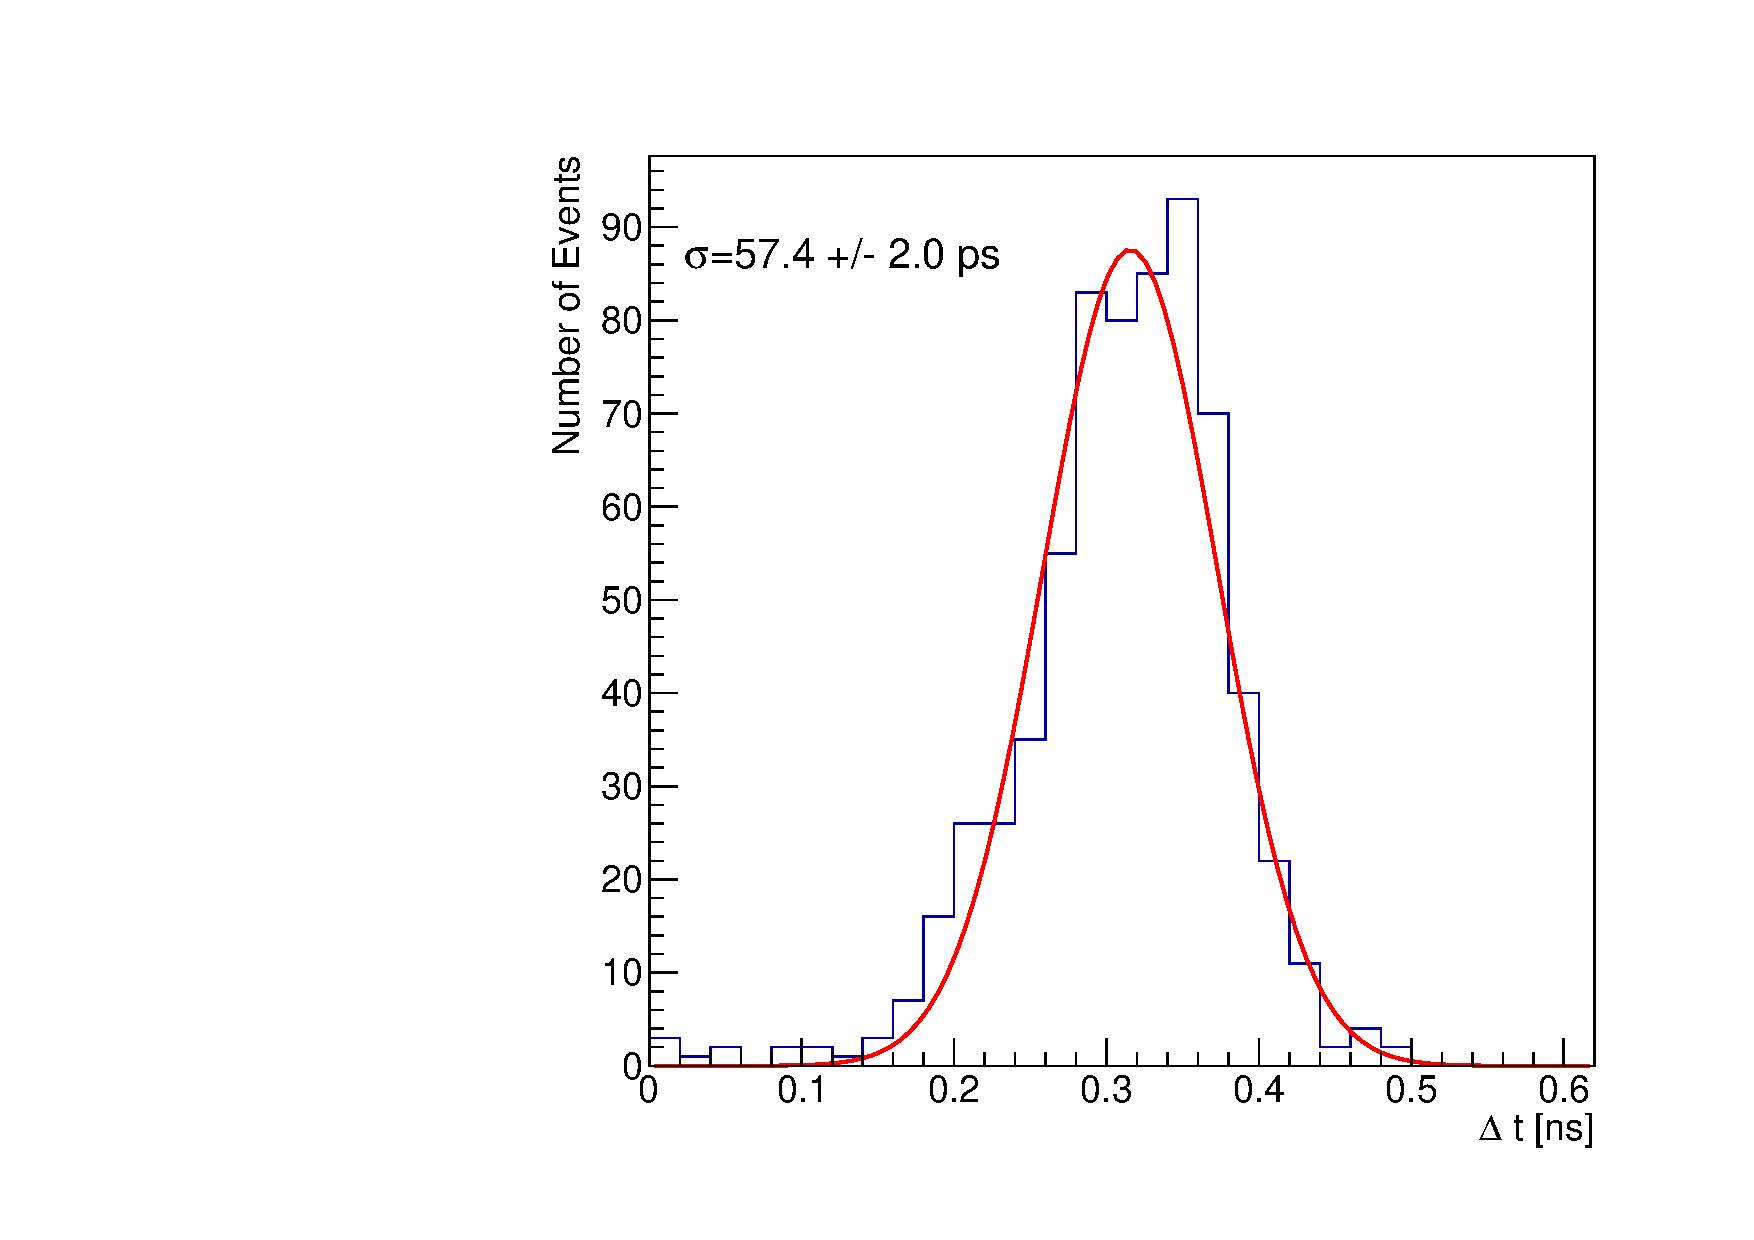
\includegraphics[width=0.45\textwidth]{figs/TOF_Electron_LYSOCube_8GeV} 
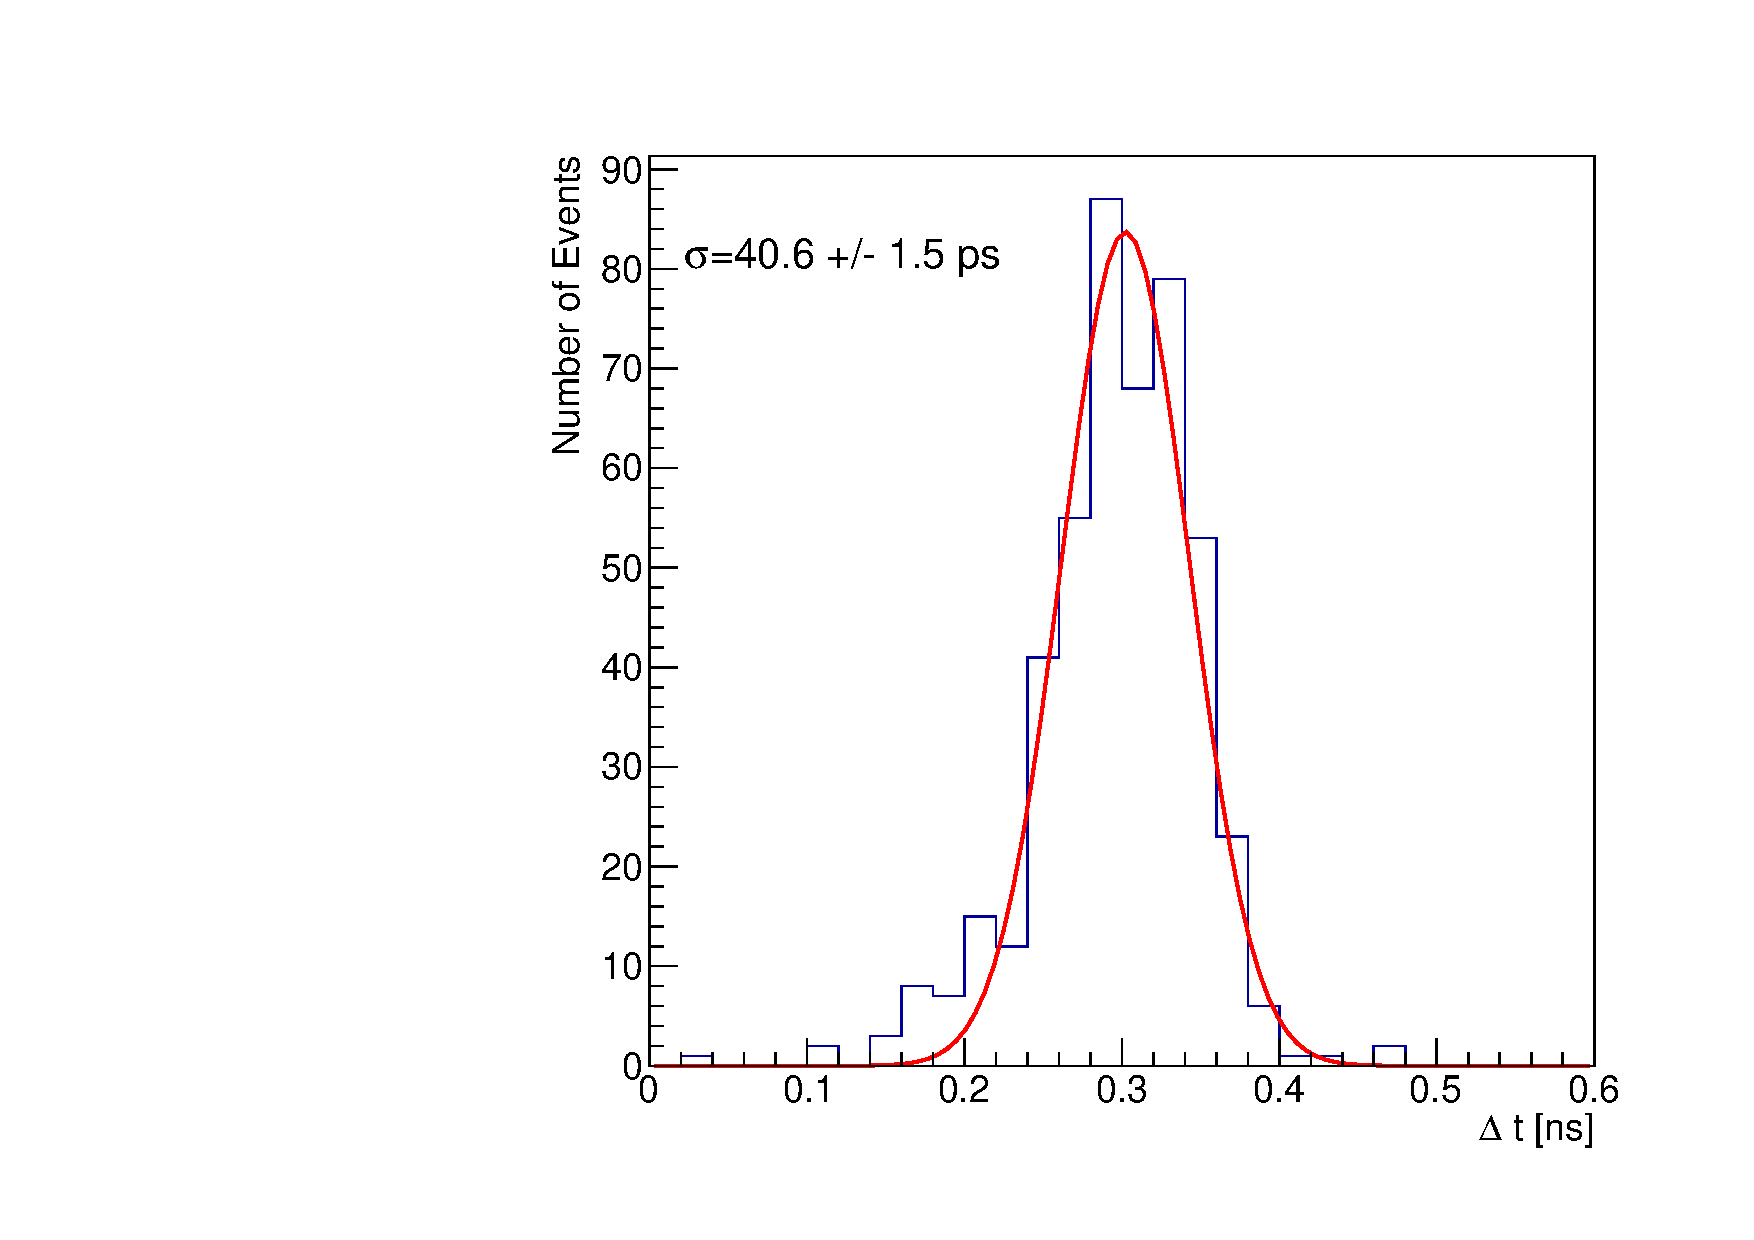
\includegraphics[width=0.45\textwidth]{figs/TOF_Electron_LYSOCube_16GeV} 
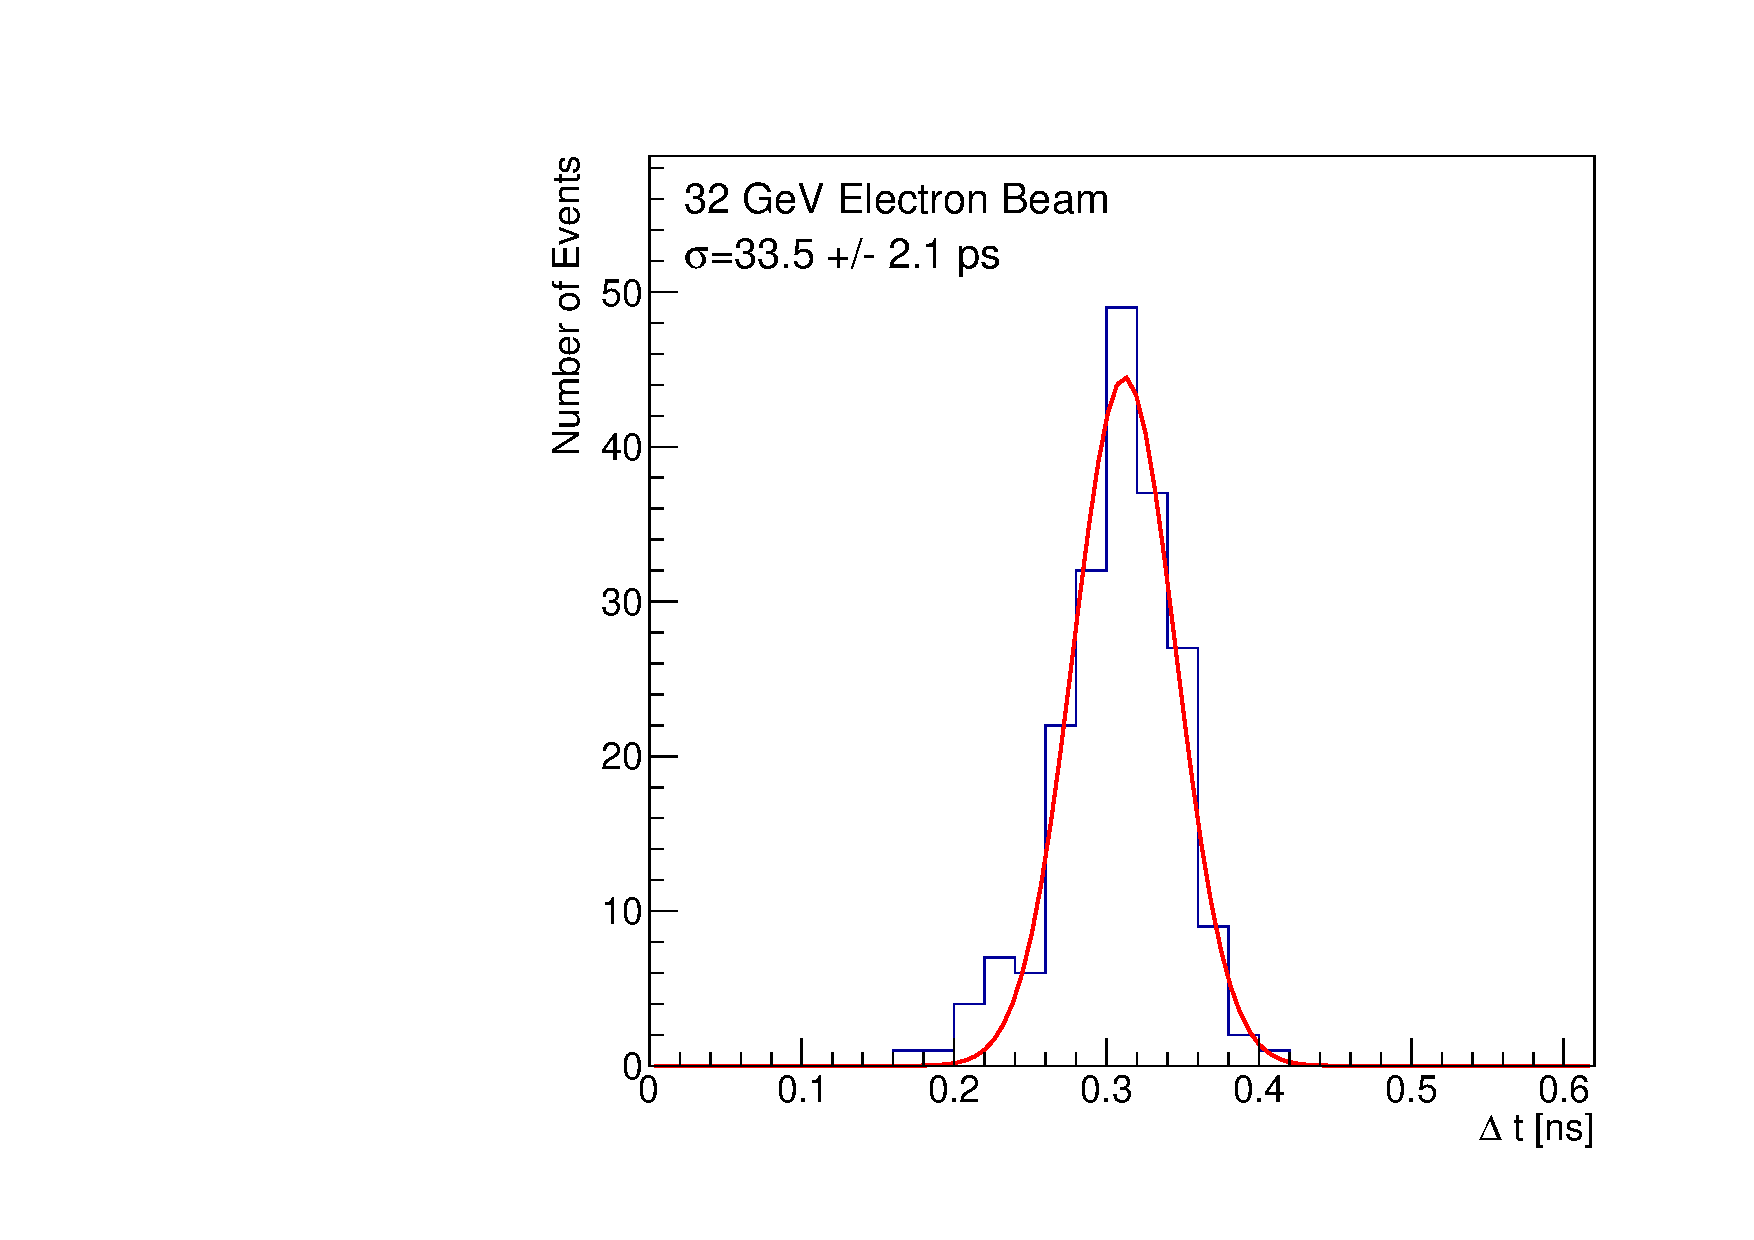
\includegraphics[width=0.45\textwidth]{figs/TOF_Electron_LYSOCube_32GeV} 
\caption{ Time of flight distributions for the LYSO cube sampling calorimeter
for electron beams with varying beam energies. } 
\label{fig:LYSOCubeTOF}
\end{figure}

The time of flight resolution measurements are plotted as a function of the
beam energy in Figure~\ref{fig:LYSOCubeTOFResolutionVsEnergy}, and is observed
to follow a $1/\sqrt{E}$ dependence. We fit the result to the sum of a 
$1/\sqrt{E}$ term and a constant term, and determine the constant term to
be about $11$~ps with an uncertainty of about $30\%$. 

\begin{figure}[h] \centering
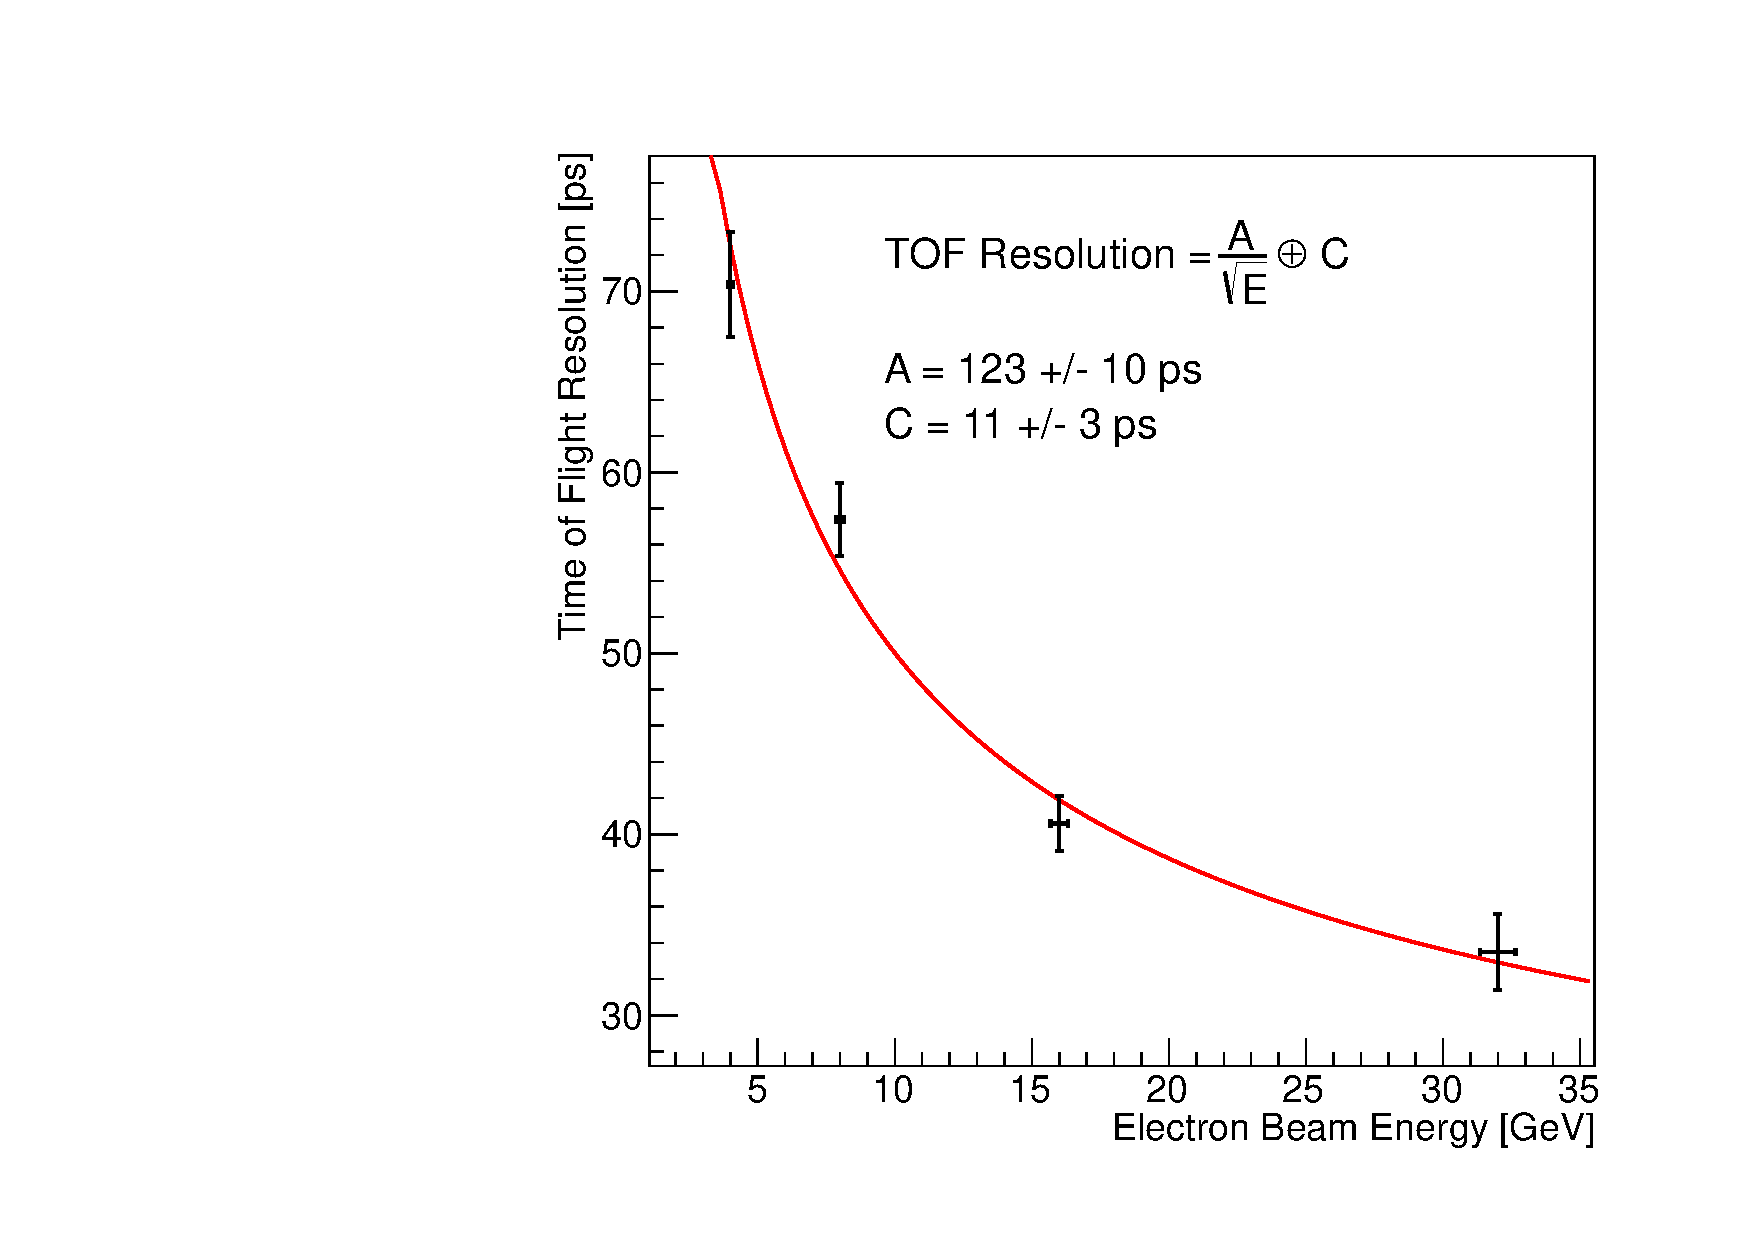
\includegraphics[width=0.45\textwidth]{figs/TimeResolutionVsEnergy_CrystalCube} 
\caption{ The time of flight resolution measured using the LYSO cube
sampling calorimeter is plotted as a function of the electron beam energy, 
and fitted to the sum of a $1/\sqrt{E}$ term and a constant term. }
\label{fig:LYSOCubeTOFResolutionVsEnergy}
\end{figure}

Given that we control the combined contribution to the time of flight
resolution of the electromagnetic shower
fluctuations, the photodetector time resolution, and the DAQ electronics
to about $25$~ps~\cite{RonzhinNIMA} and that the geometric contribution 
from the transverse size of the trigger is about $12$~ps,
we infer that the contribution of the scintillation mechanism in LYSO
to the time of flight resolution is less than $20$~ps.


\subsection{Studies of Time Jitter from Optical Transport}

We study the contribution to the time of flight resolution due to
various forms of optical transport in the context of a LYSO-tungsten Shashlik
calorimeter, one of the proposed choices for the Phase 2 upgrade of the
CMS endcap calorimeter system. We compare the time of flight resolution
performance for two alternative optical transport schemes. 

We begin with a conventional scheme where scintillation light is collected
by wavelength shifting fibers through a set of four holes penetrating 
the LYSO layers. A schematic diagram and a photograph showing this setup 
is shown in Figure~\ref{fig:ShashlikFiberSetup}. 
MCP photomultiplier tubes produed by Hamamatsu (R3809) are used to collect 
the scintillation light, while a Photek 240 MCP is used as the reference 
time detector. 


\begin{figure}[h] \centering
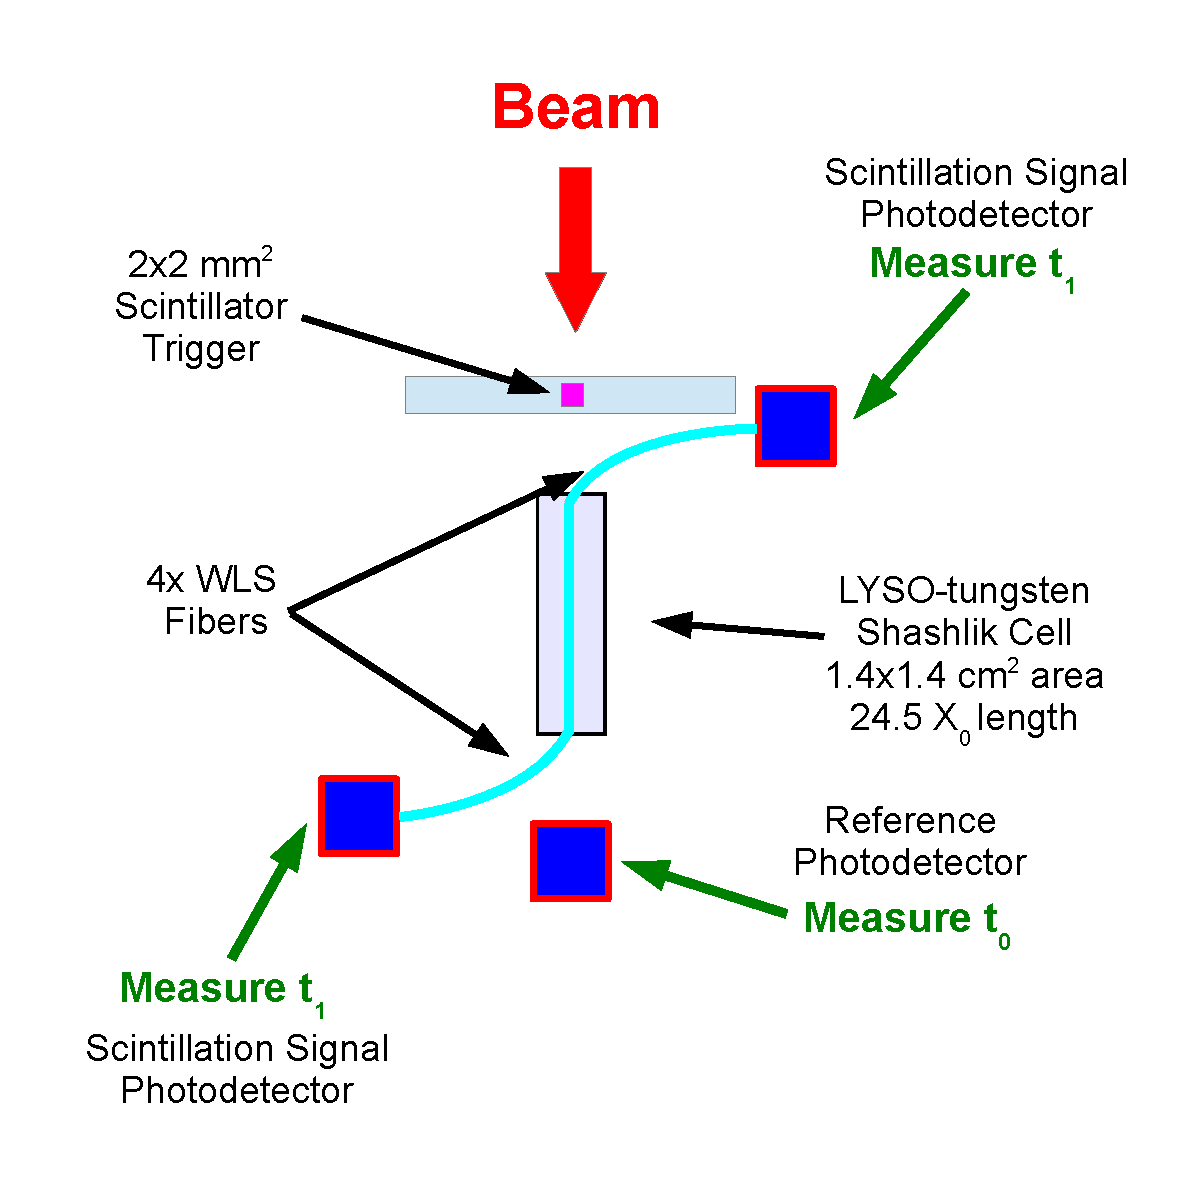
\includegraphics[width=0.45\textwidth]{figs/ShashlikFiberSetupSchematic} 
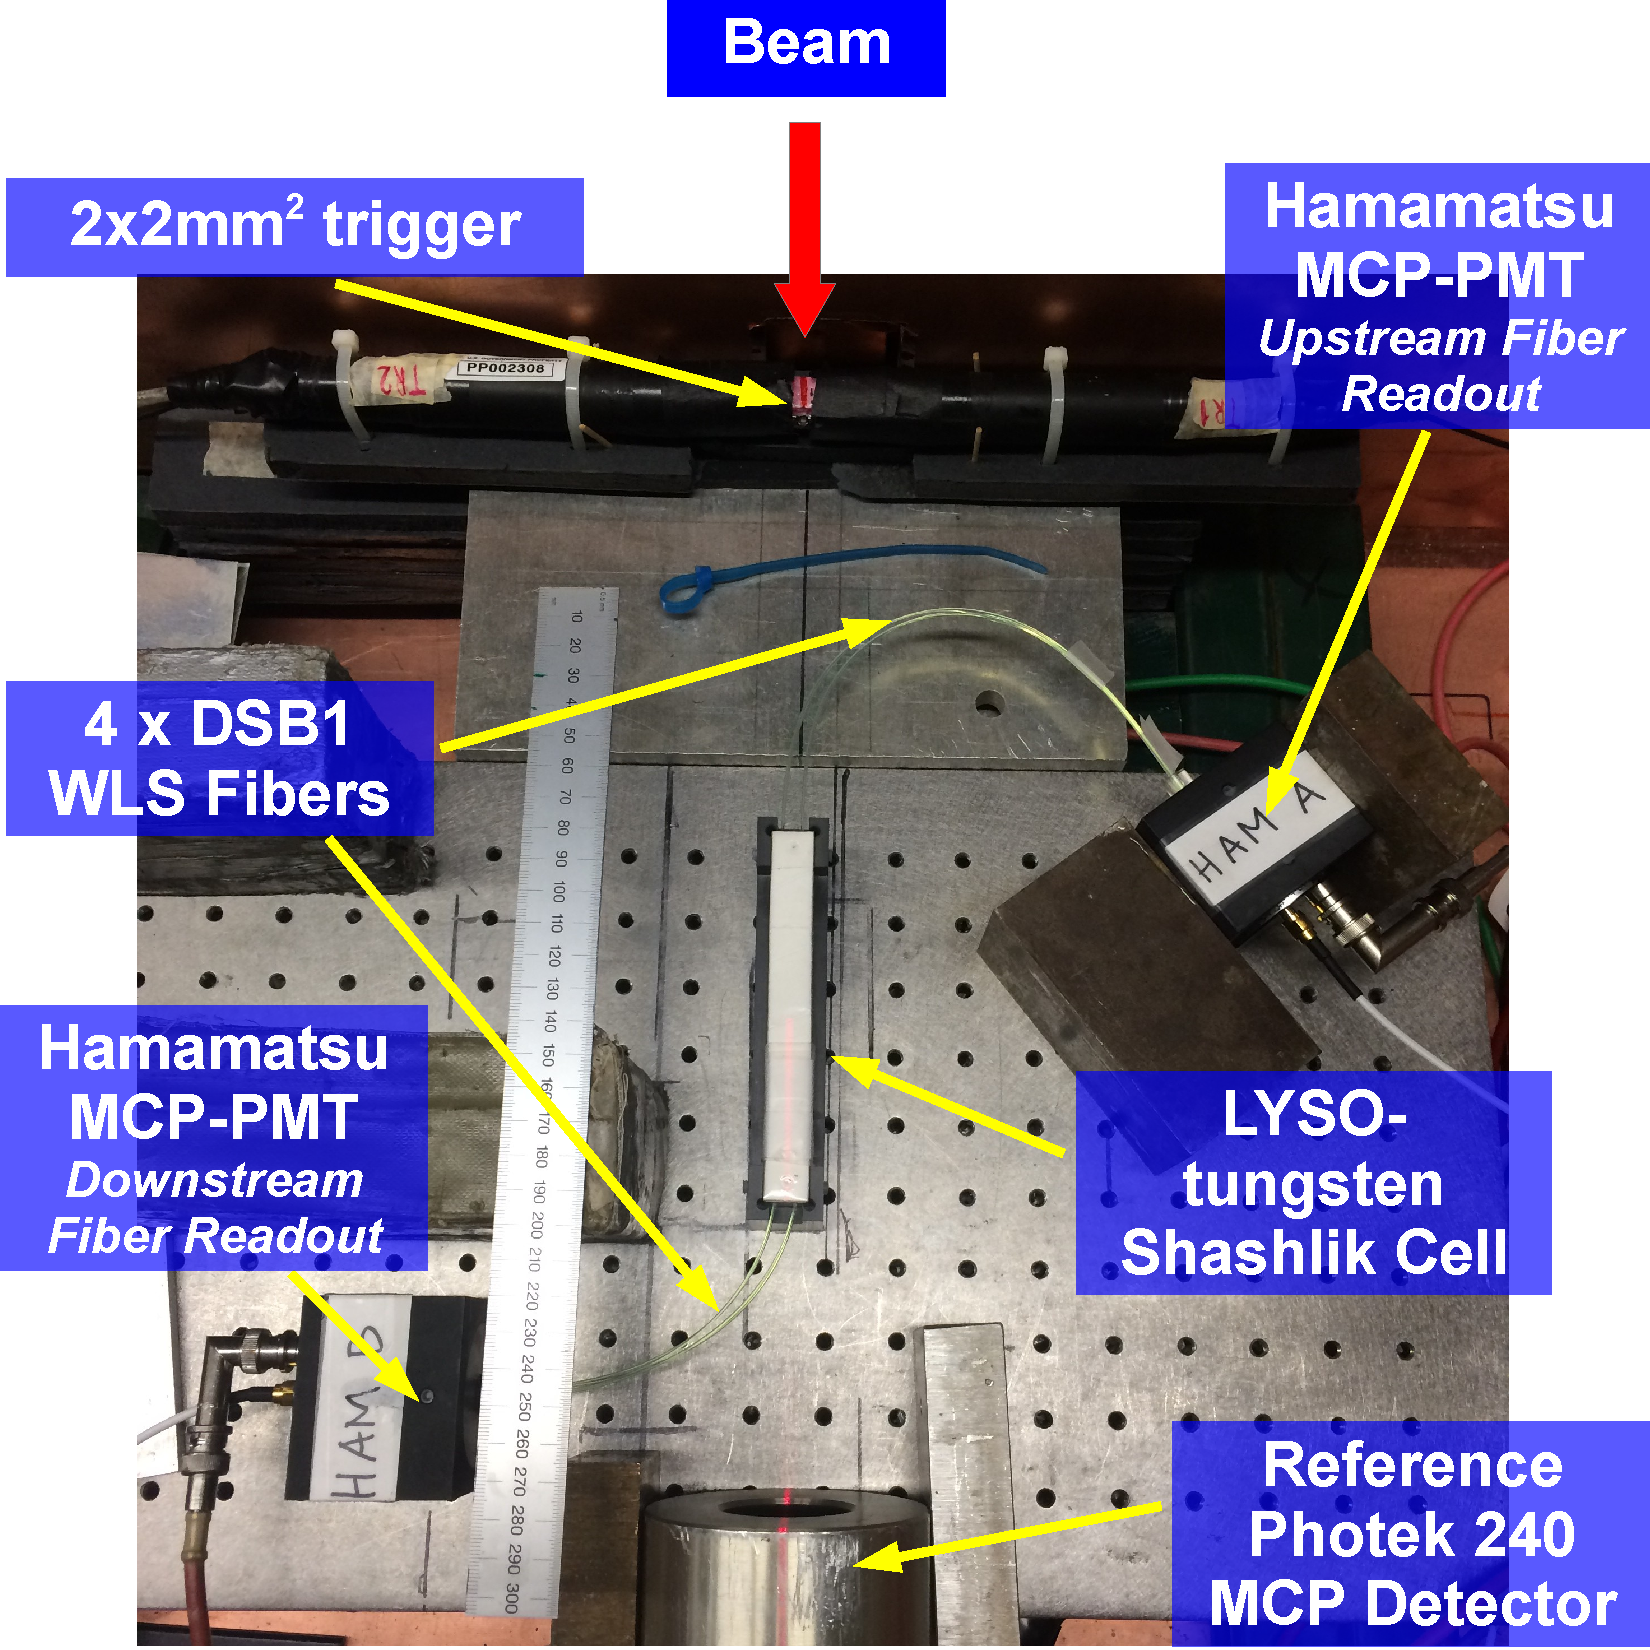
\includegraphics[width=0.45\textwidth]{figs/ShashlikFiberSetupPhoto} 
\caption{ A schematic diagram of the experimental setup for the
time of flight measurement using the LYSO-tungsten shashlik calorimeter
with fiber signal extraction is shown, along with a photograph of the
experimental setup. } 
\label{fig:ShashlikFiberSetup}
\end{figure}

In addition to effects of light transport along the fiber, 
this scheme has the added effect of absorption and re-emission as 
the scintillation light enters the wavelength shifting material. 
The characteristic time scales involved in the wavelength shifting 
mechanism may affect the rise time and time jitter of the final signal 
pulse. We investigate this particular effect in greater detail by
comparing the signal pulses obtained using two different types
of wavelength shifting fiber in the same LYSO-tungsten shashlik
calorimeter. In Figure~\ref{fig:FiberPulseComparison} we show
the pulse shapes averaged over a few hundred events obtained 
using DSB1 fibers and Y11 fibers, plotted in blue and red respectively,
compared with the average pulse shape obtained from direct optical 
coupling to the edge of one of the LYSO tiles, plotted in green.
We find that the rise time of the pulse shape obtained using the 
DSB1 fibers, at about $3.5$~ns, is significantly faster than the rise time
of the pulse obtained using the Y11 fibers, which is about $10$~ns,
and is within a factor of two of the rise time for the pulse obtained 
through direct optical coupling to the photodetector. This indicates
that the choice of fiber is an important parameter for 
optimizing the time of flight resolution for the design of 
this type of calorimeter, and that the DSB1 fibers 
already provides a reasonably good choice.

\begin{figure}[h] \centering
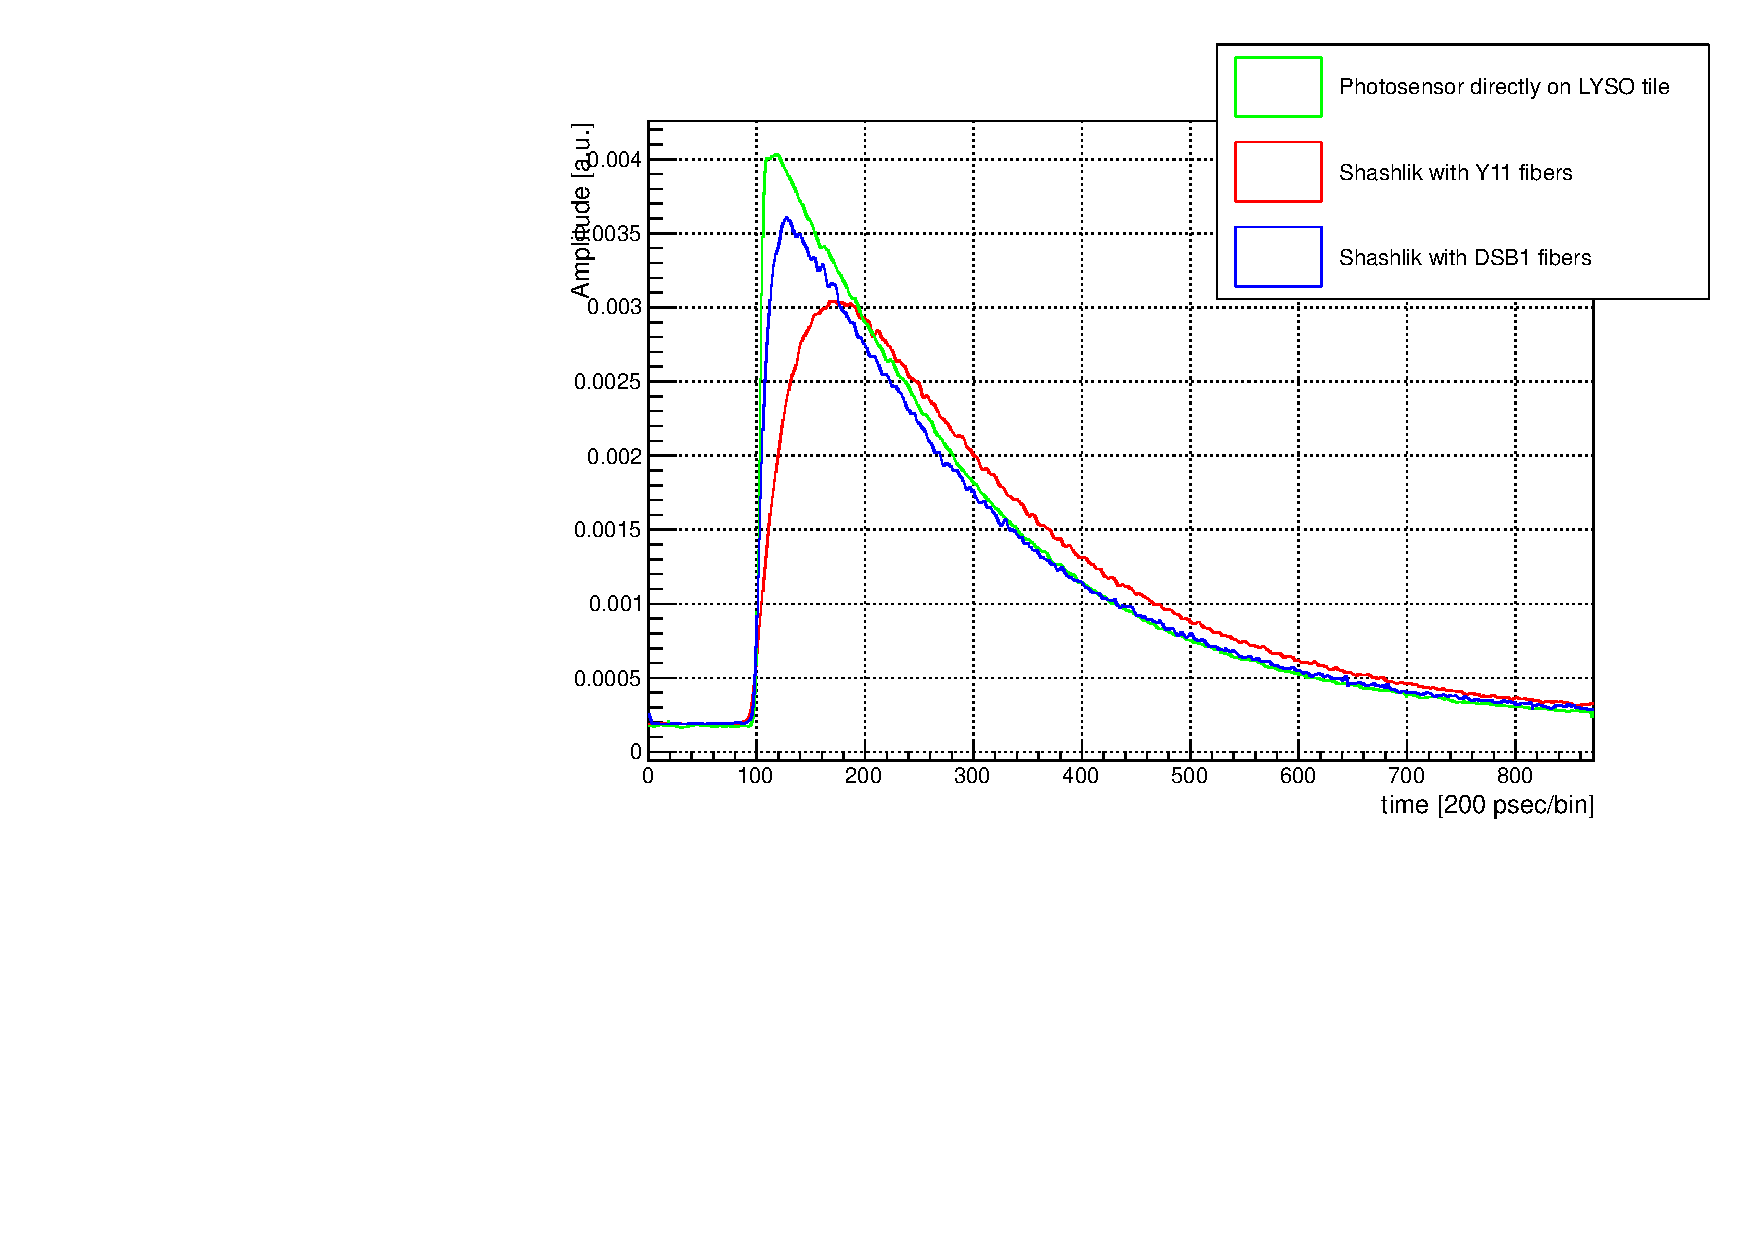
\includegraphics[width=0.45\textwidth]{figs/FiberPulses} 
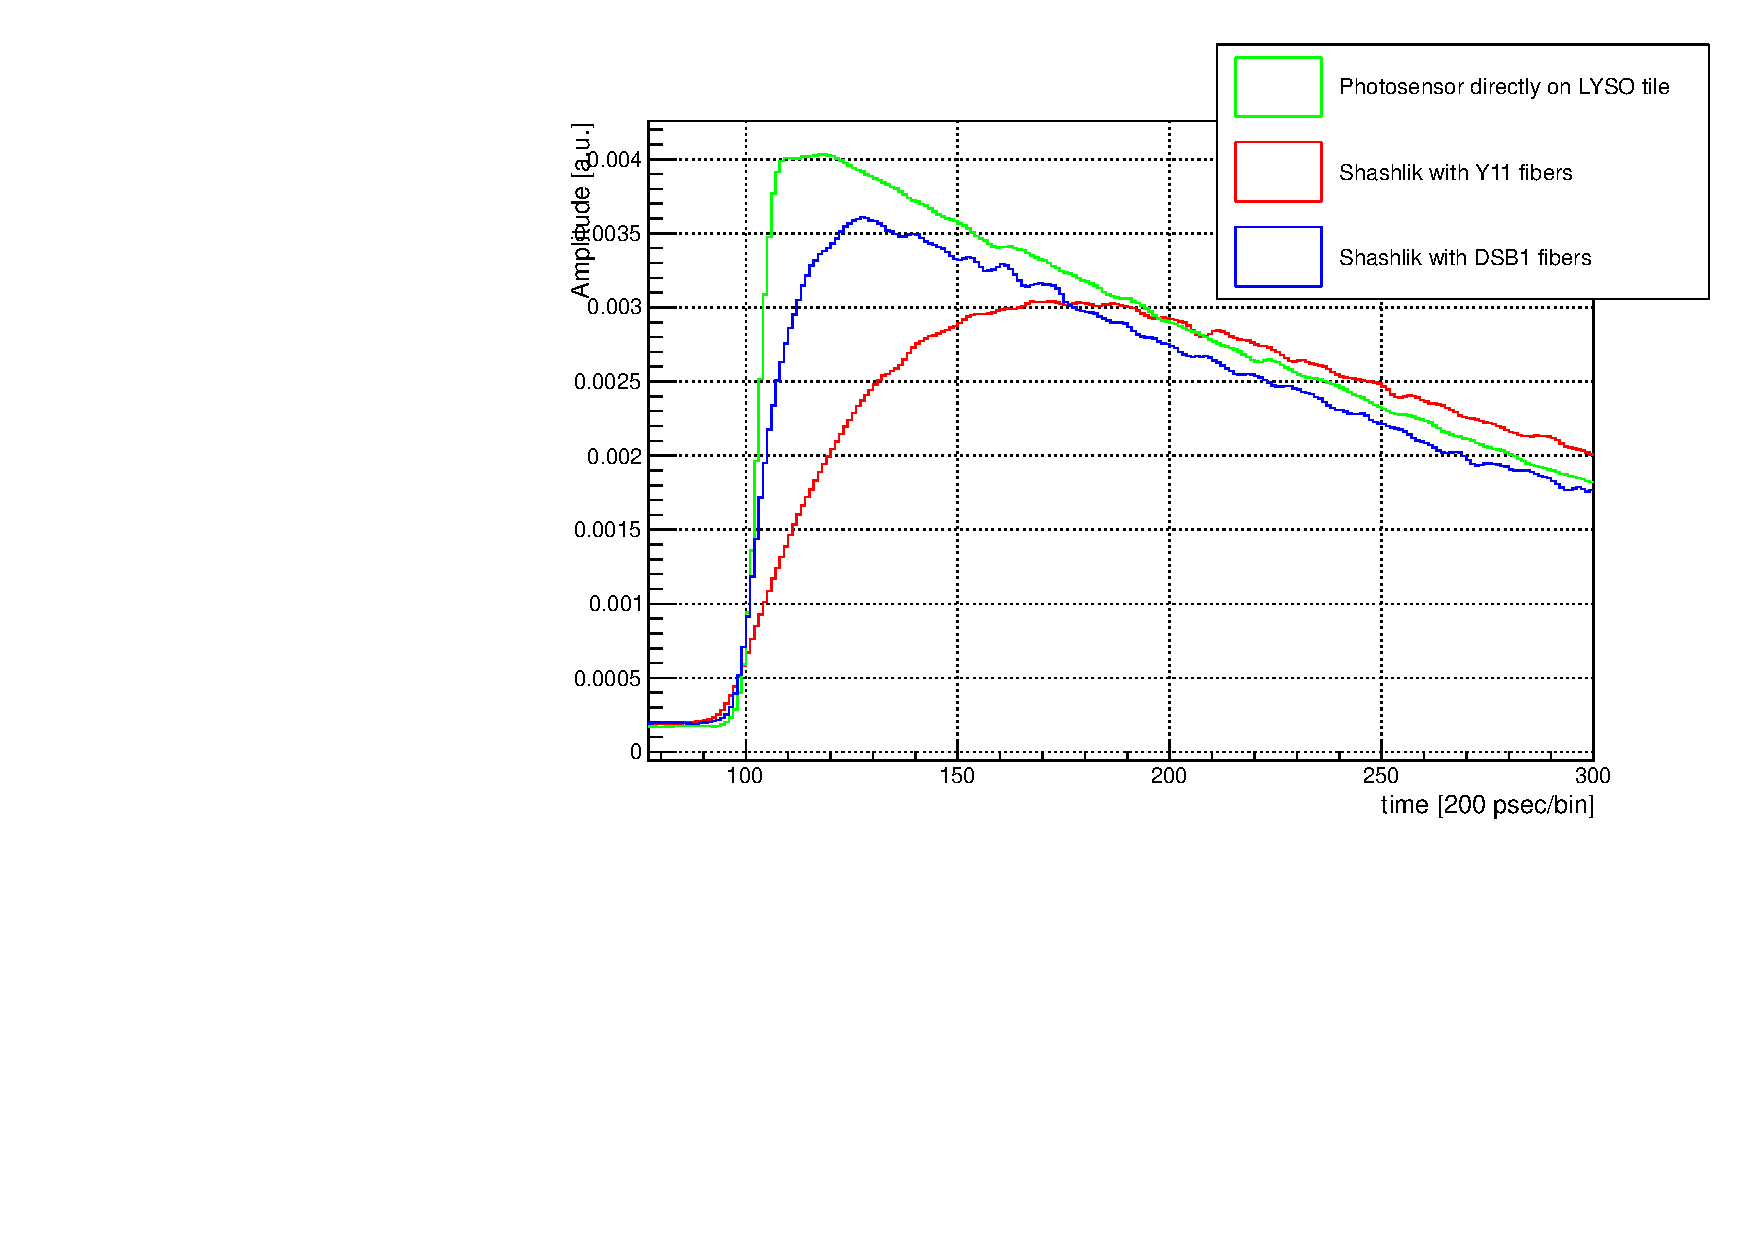
\includegraphics[width=0.45\textwidth]{figs/FiberPulsesZoom} 
\caption{ Pulse shapes digitized by the DRS4 board and averaged over several hundred events 
obtained from the LYSO-tungsten shashlik calorimeter with light extracted using
DSB1 (blue) and Y11 (red) wavelength shifting fibers, are compared with 
the averaged pulse shapes obtained from direct coupling of the photodetector (green)
to one edge of one of the LYSO tiles in the shashlik calorimeter.} 
\label{fig:FiberPulseComparison}
\end{figure}


Using the DSB1 fibers, we measure the time of flight resolution
for electron beams with beam energy varying between $4$~GeV and $32$~GeV.
In Figure~\ref{fig:ShashlikFiberEnergy32GeV} we show the distribution
of the pulse integral, a quantity proportional to the measured energy,
for the $32$~GeV beam and observe an energy resolution of about $5\%$.
The time of flight distributions, fitted to gaussian functions,
are shown in Figure~\ref{fig:ShashlikFiberTOF}, and the resulting
$\sigma$ parameter of the gaussian is plotted as a function of the
beam energy in Figure~\ref{fig:ShashlikFiberTOFResolutionVsEnergy}.
We find that the dependence of the time of flight resolution on
beam energy exhibits a $1/\sqrt{E}$ functional form, indicating
that the current calorimeter setup remains in the photo-statistics
limited regime. The best time of flight resolution we obtain
with this setup is about $110$~ps. As the measurement is photo-statistics
limited, to improve on this result in the future, work is needed
on improving the light collection efficiency. 

\begin{figure}[h] \centering
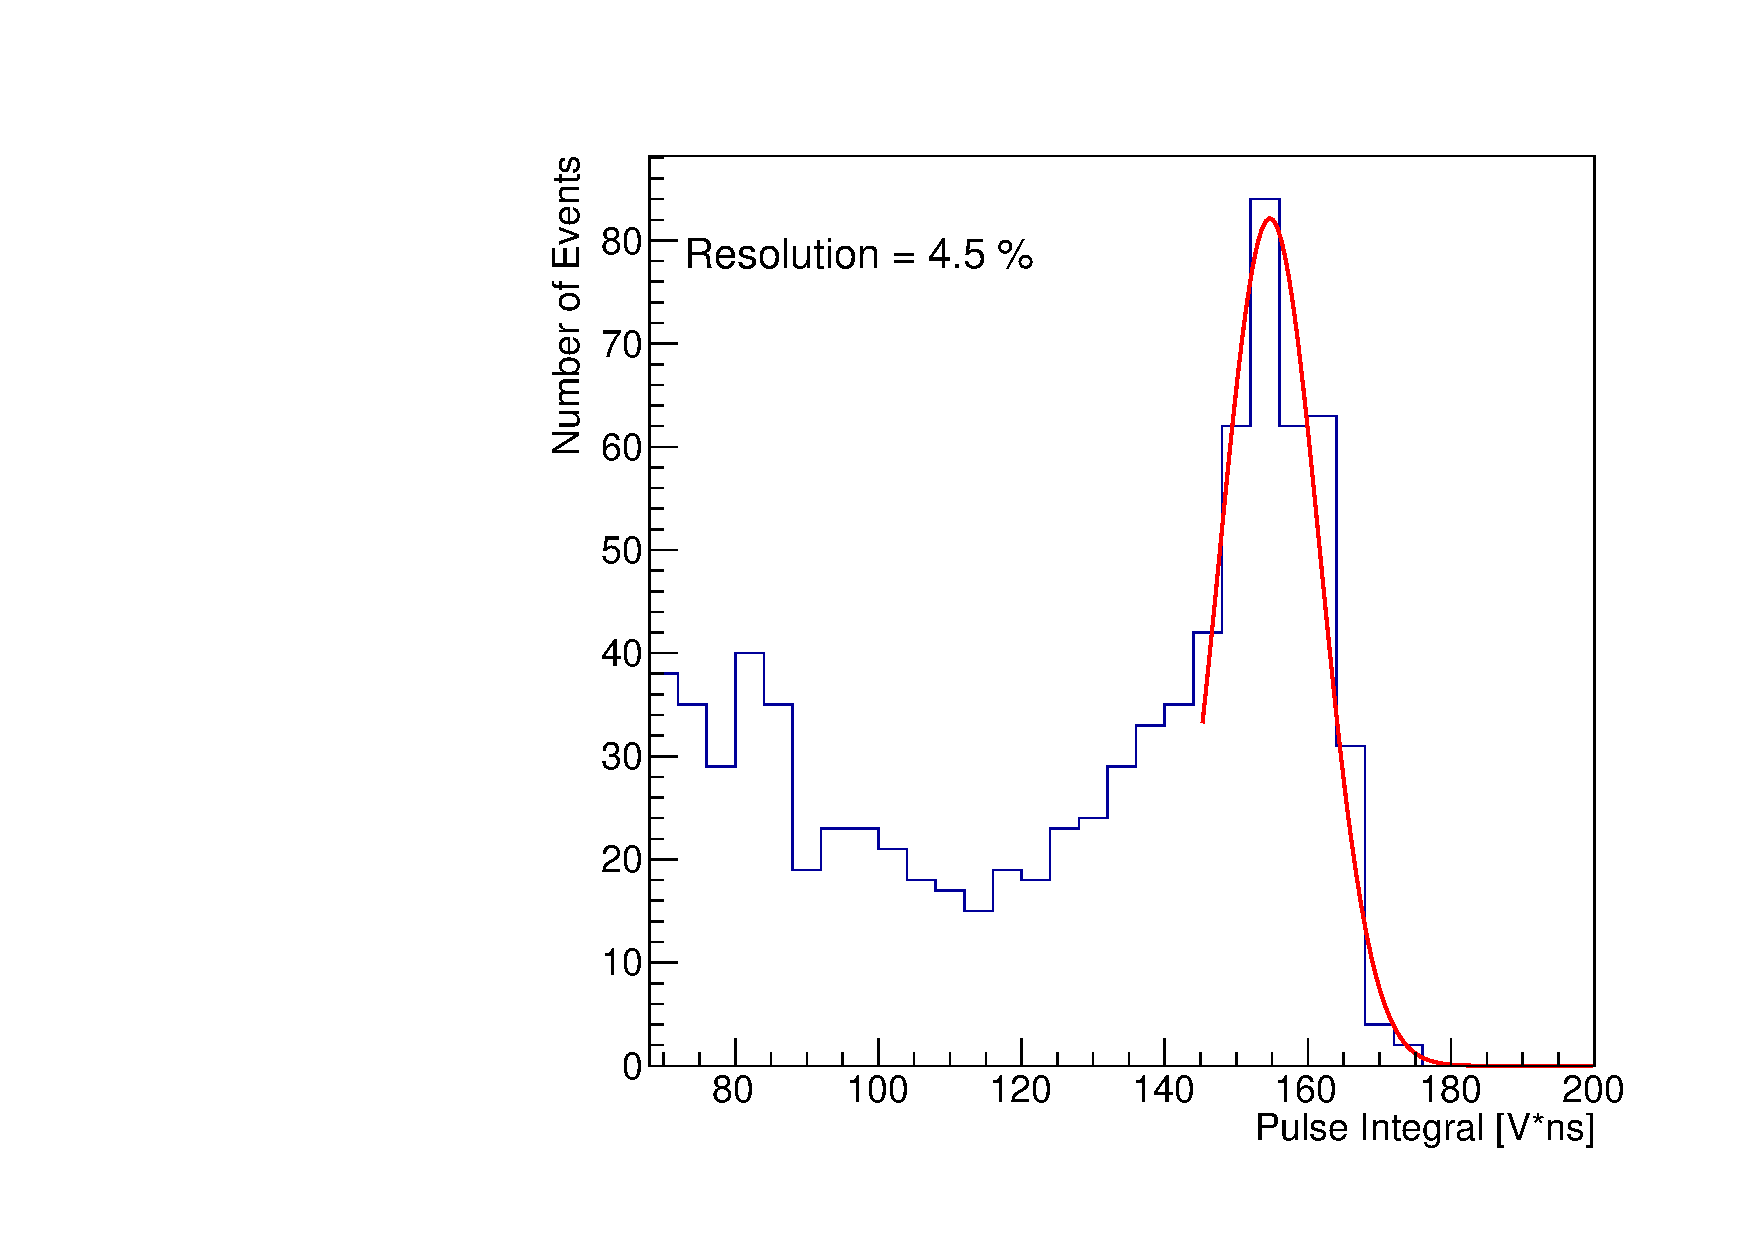
\includegraphics[width=0.45\textwidth]{figs/TOF_ShashlikDSB1Fiber_Electron_32GeV_energy} 
\caption{ Histogram of the pulse integral for events recorded using
the LYSO-tungsten shashlik calorimeter using the DSB1 fibers for 
a $32$~GeV electron beam. } 
\label{fig:ShashlikFiberEnergy32GeV}
\end{figure}

\begin{figure}[h] \centering
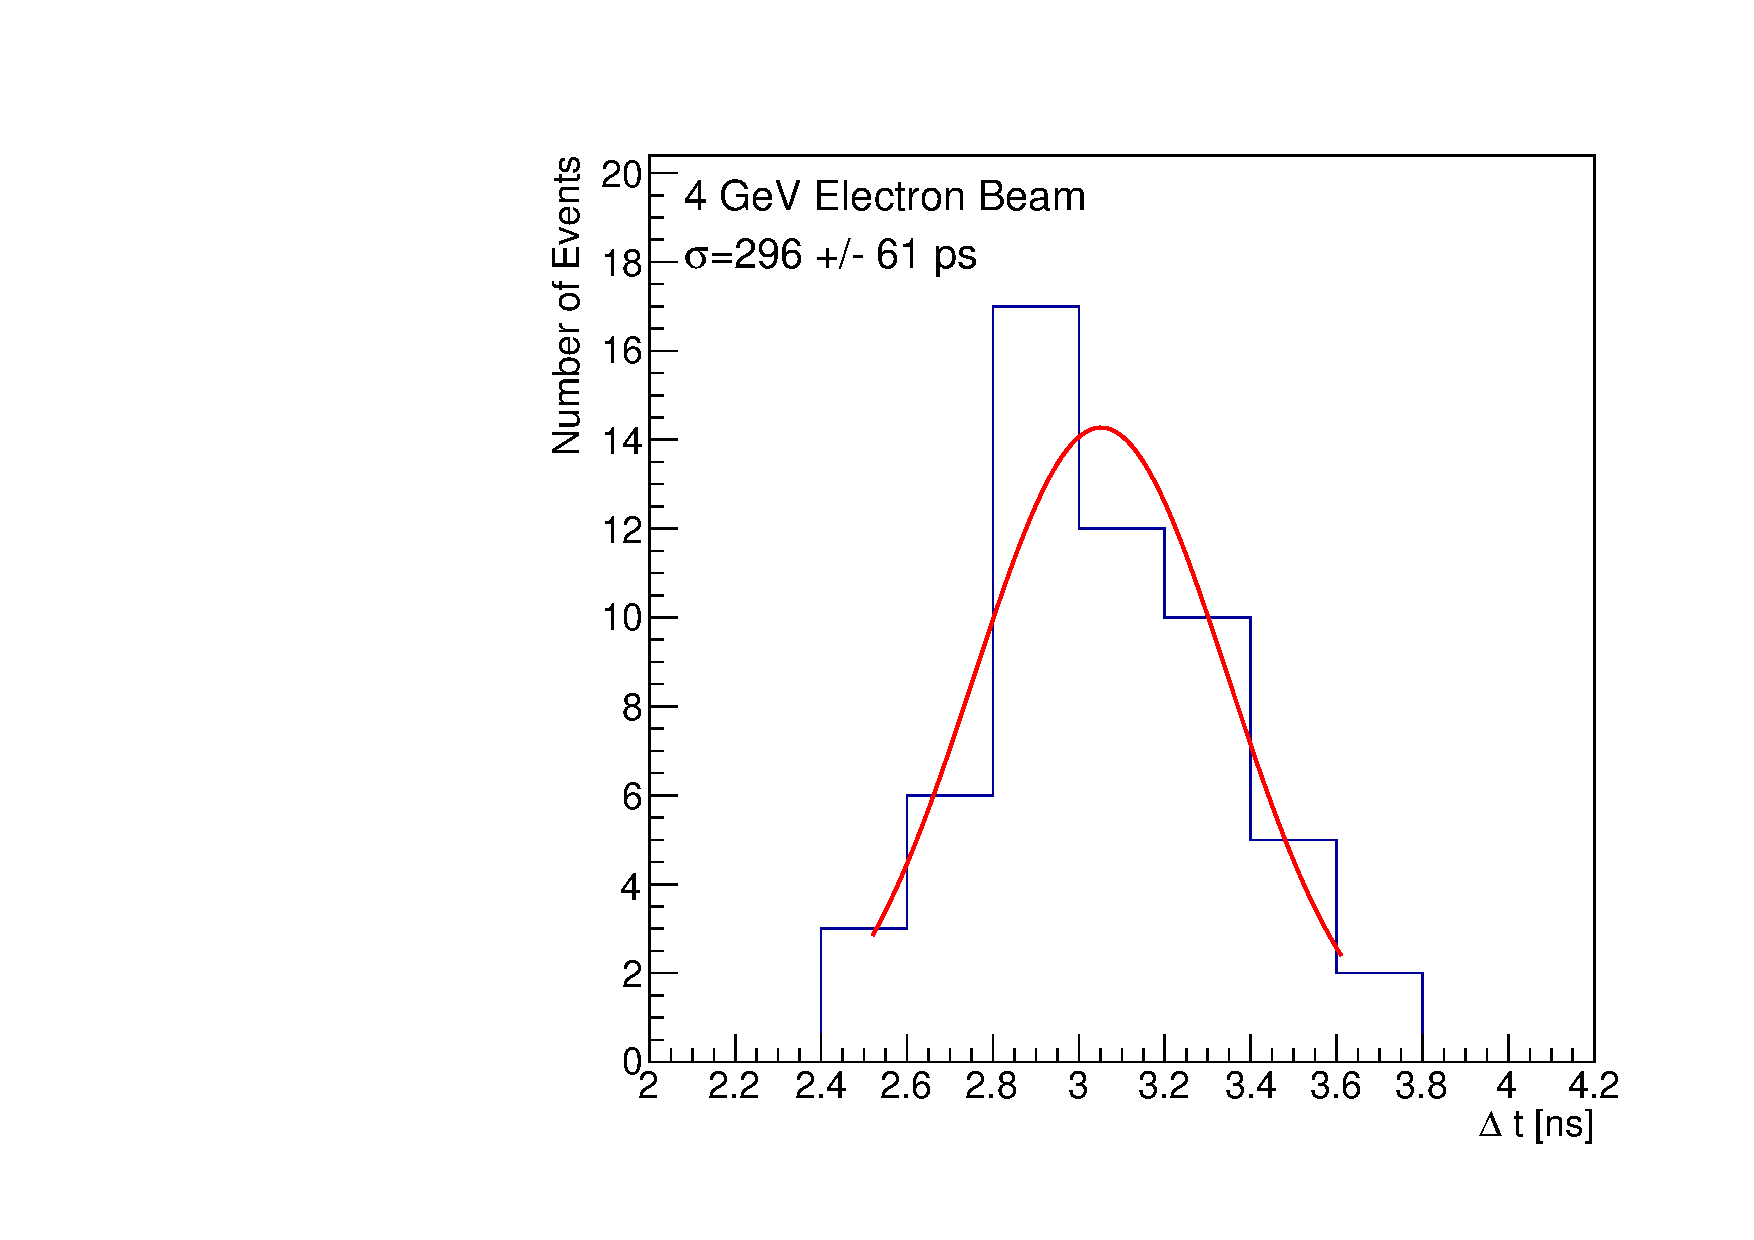
\includegraphics[width=0.45\textwidth]{figs/TOF_ShashlikDSB1Fiber_Electron_4GeV} 
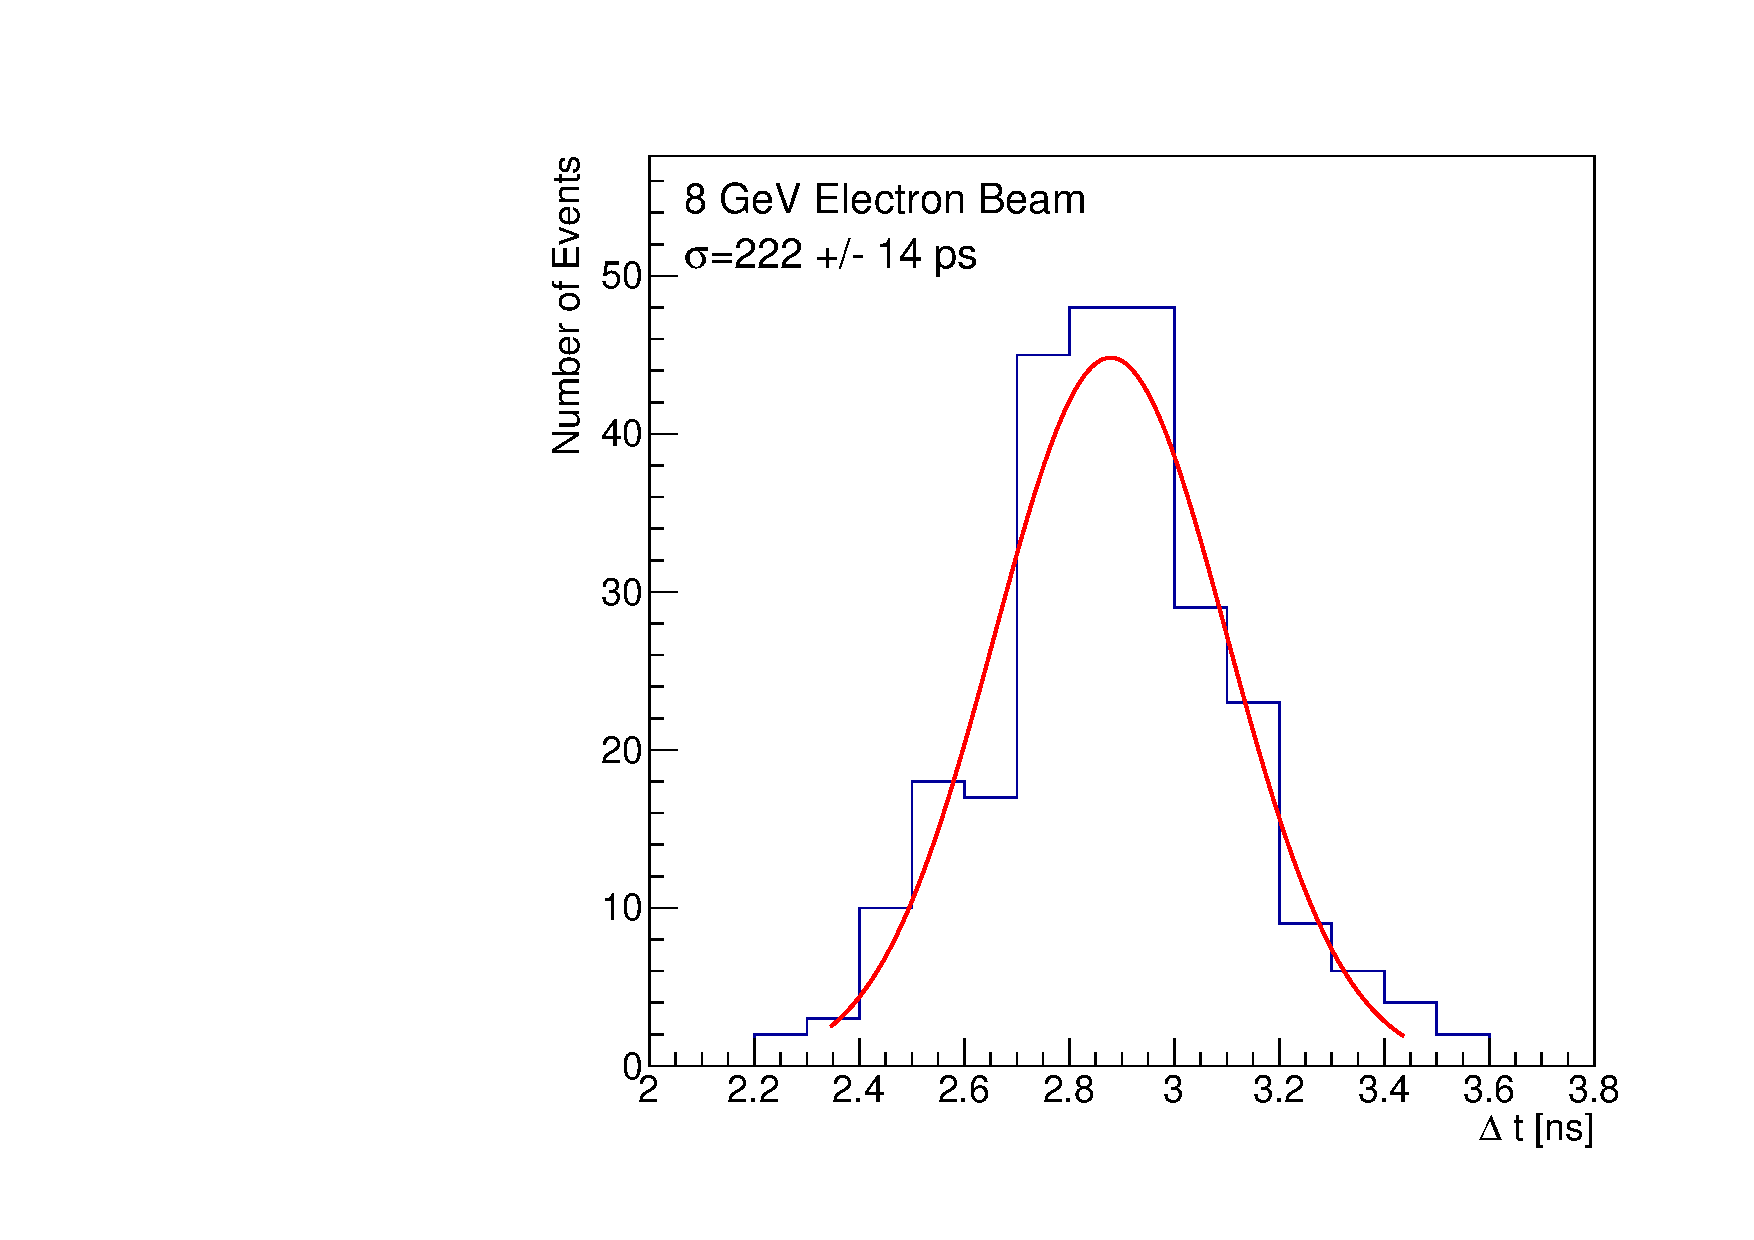
\includegraphics[width=0.45\textwidth]{figs/TOF_ShashlikDSB1Fiber_Electron_8GeV} 
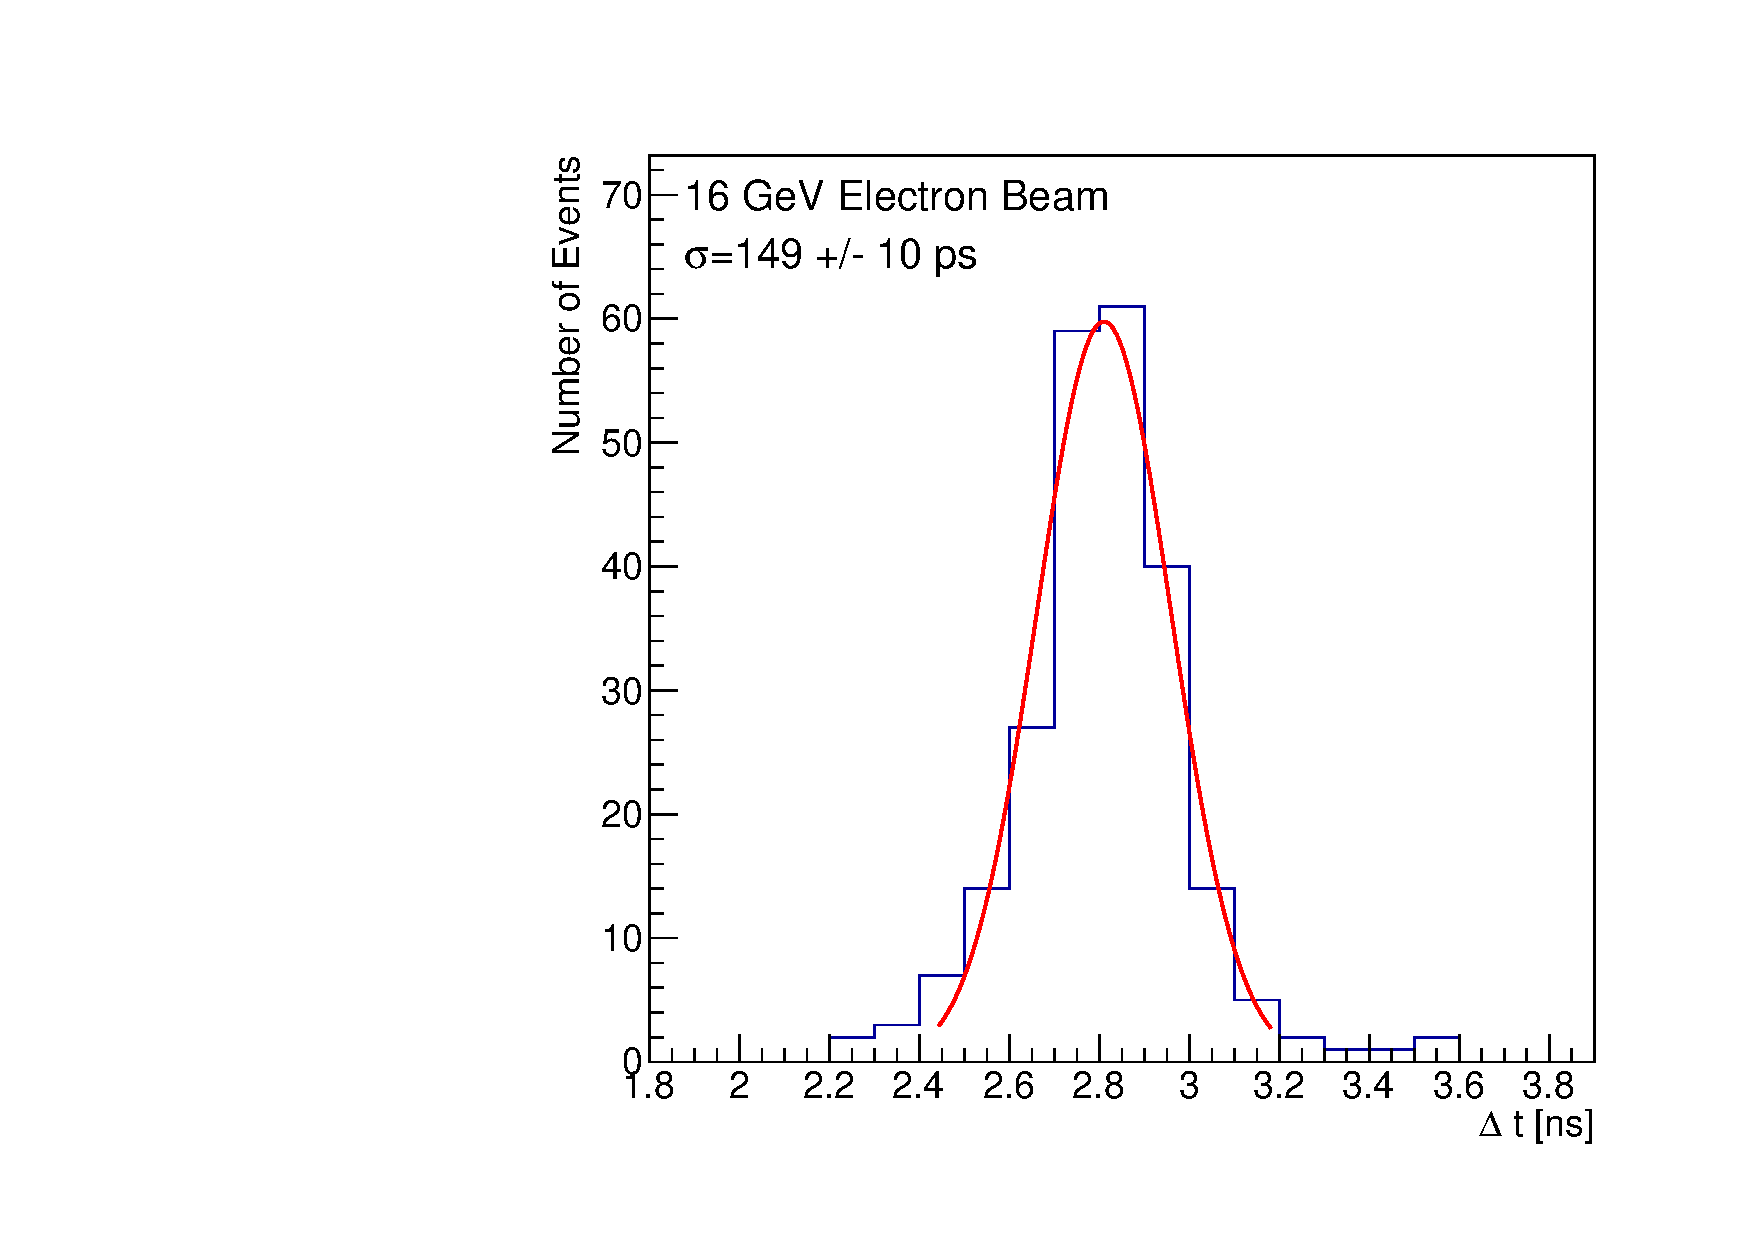
\includegraphics[width=0.45\textwidth]{figs/TOF_ShashlikDSB1Fiber_Electron_16GeV} 
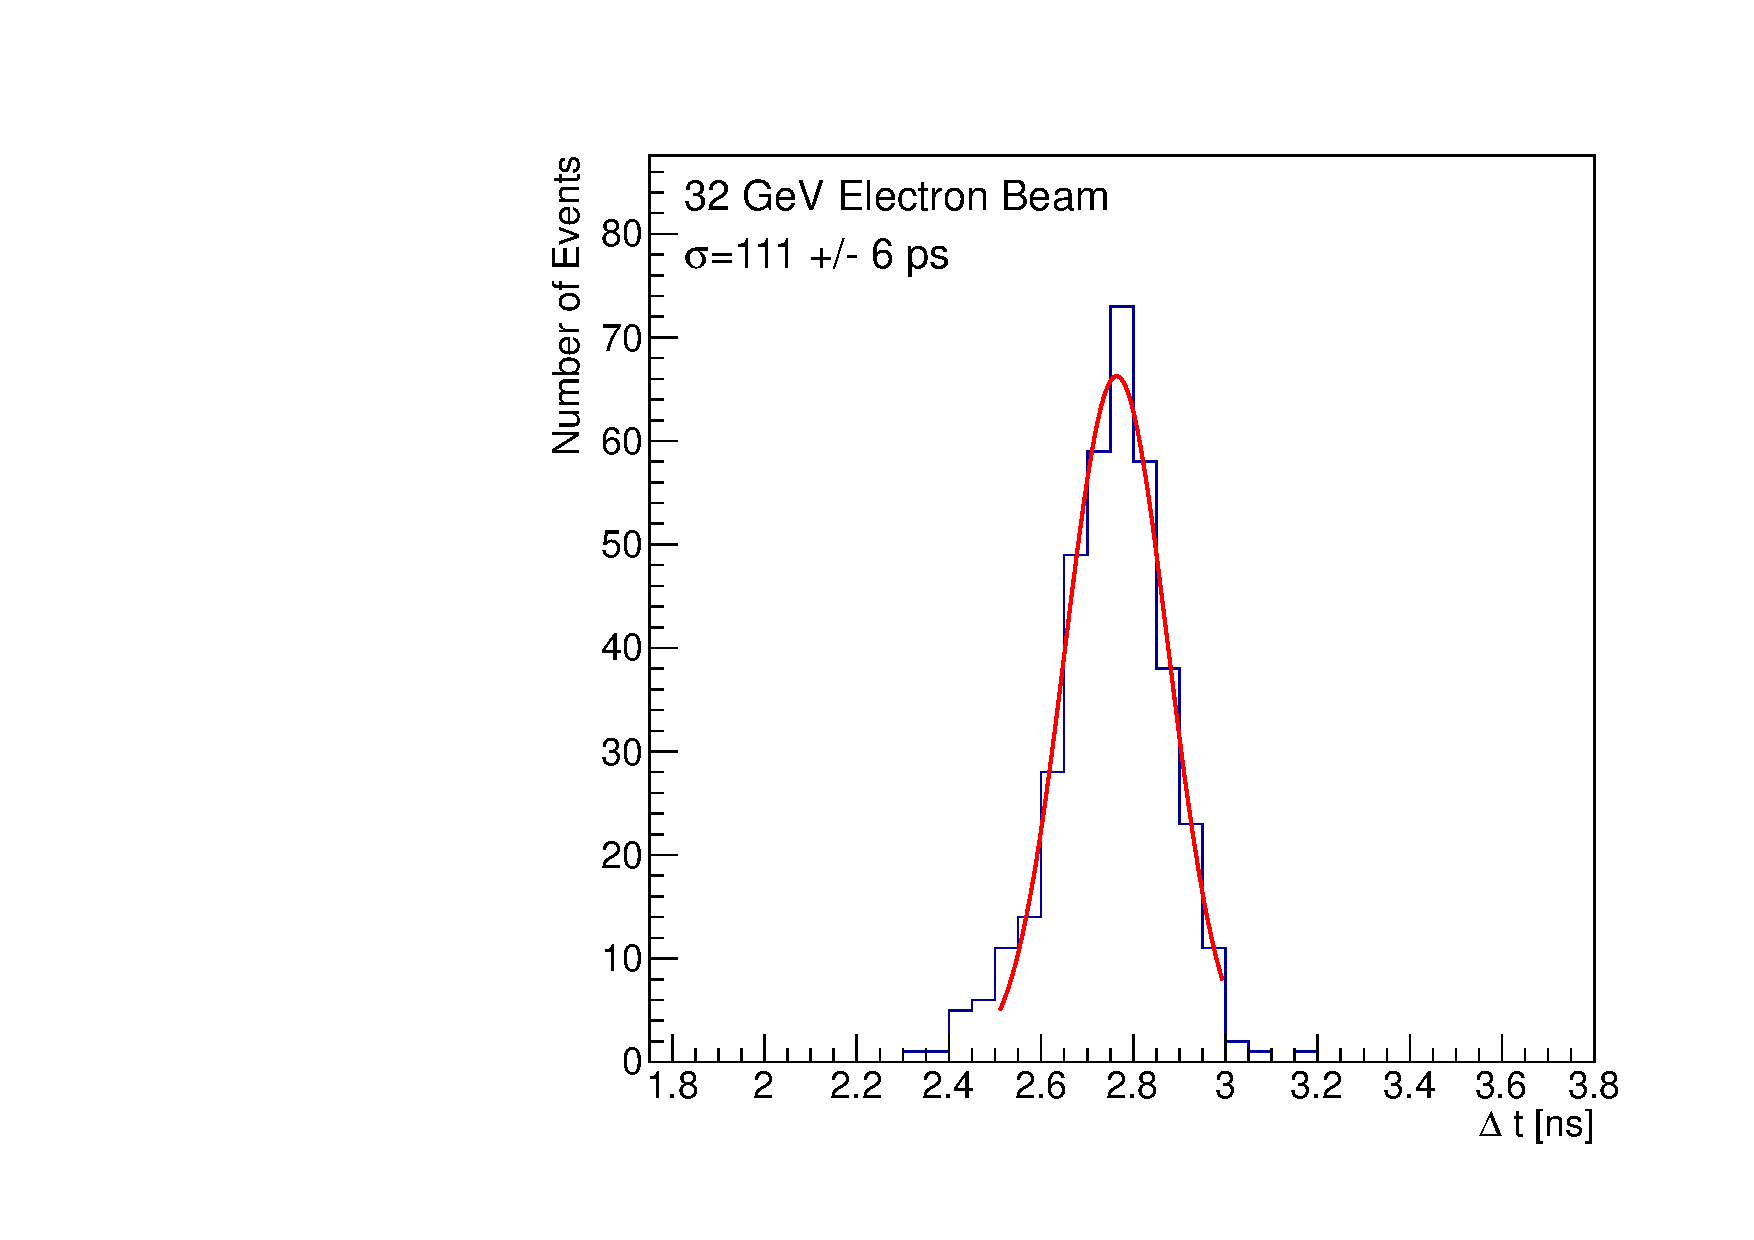
\includegraphics[width=0.45\textwidth]{figs/TOF_ShashlikDSB1Fiber_Electron_32GeV} 
\caption{ Time of flight distributions for the LYSO-tungsten shashlik calorimeter
using DSB1 fibers for electron beams with varying beam energies. } 
\label{fig:ShashlikFiberTOF}
\end{figure}

\begin{figure}[h] \centering
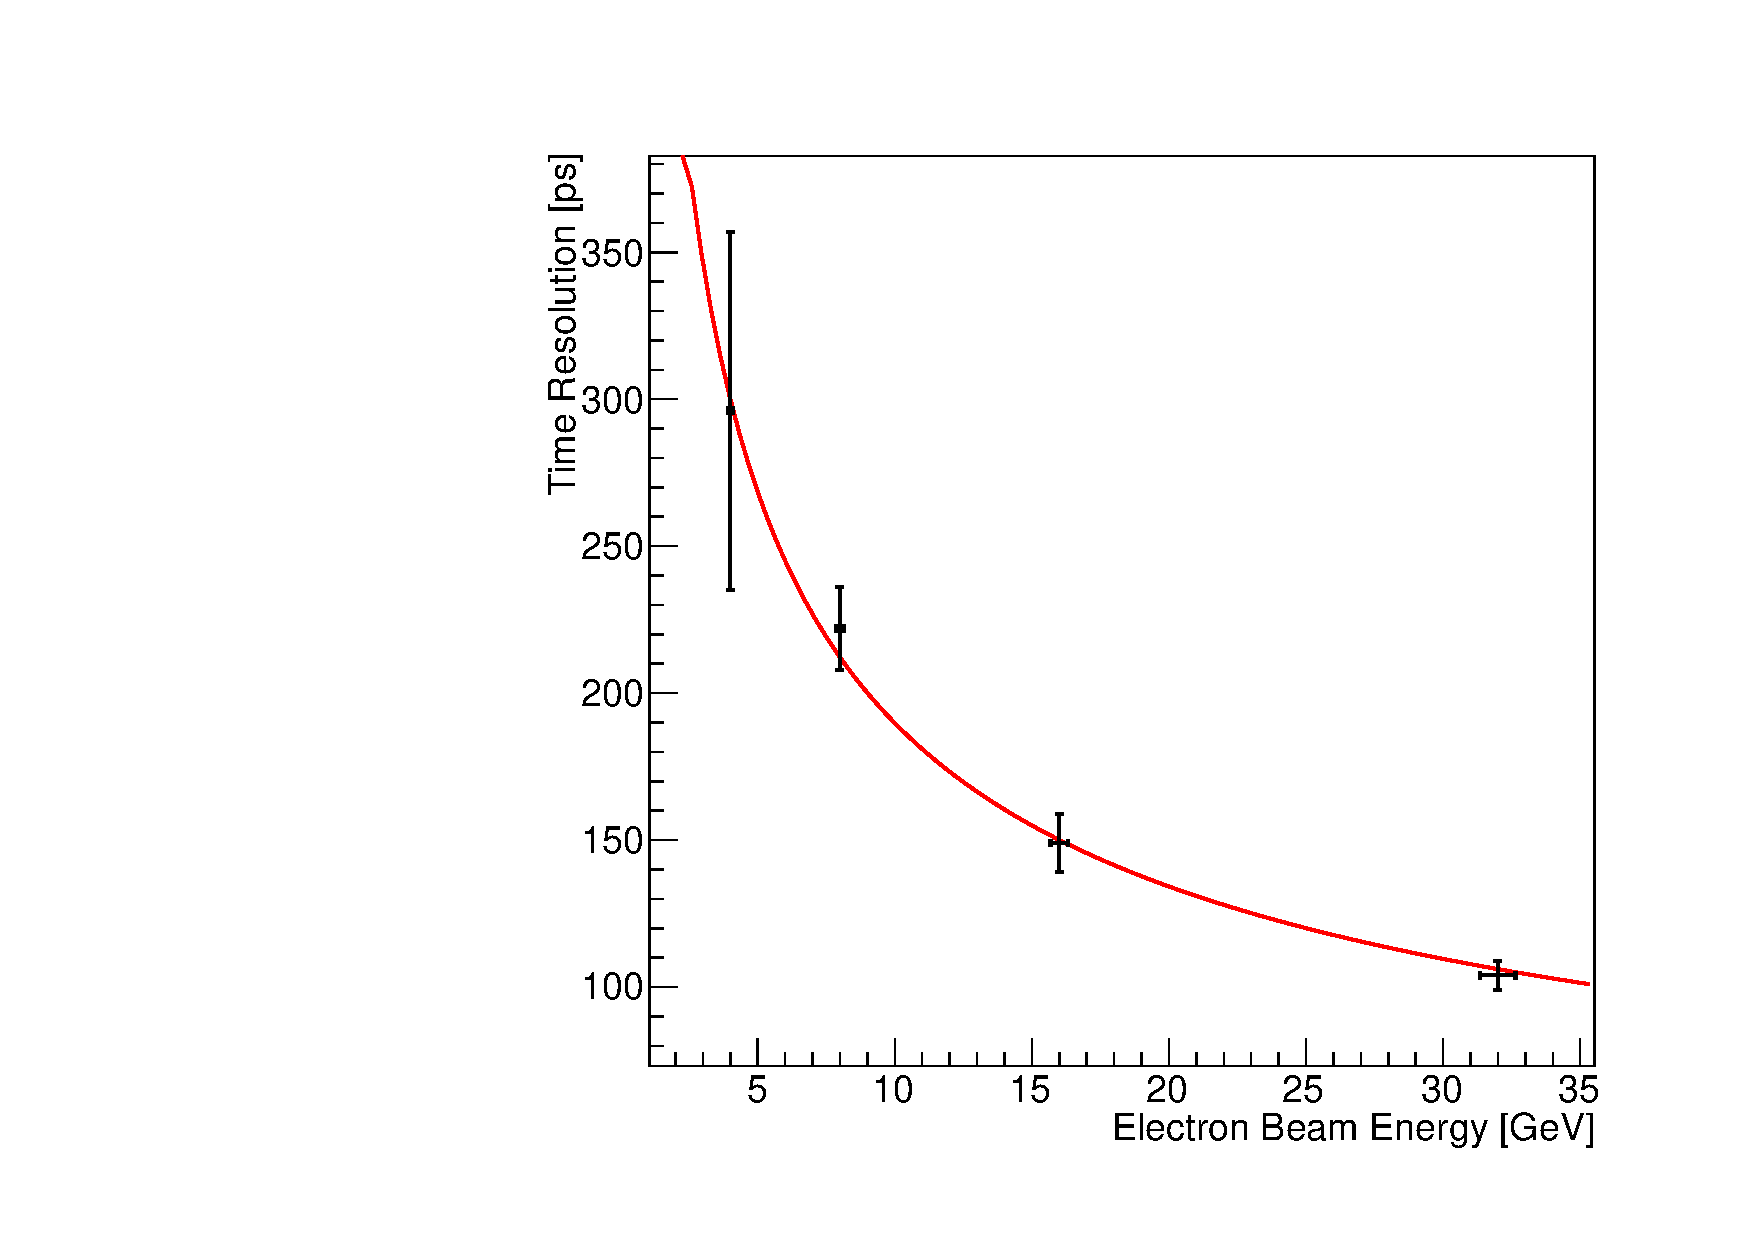
\includegraphics[width=0.45\textwidth]{figs/TimeResolutionVsEnergy_ShashlikDSB1Fiber} 
\caption{ The time of flight resolution measured using the LYSO-tungsten shashlik
calorimeter with signal extracted using DSB1 fibers is plotted as a function of
the electron beam energy, and fitted to a $1/\sqrt{E}$ functional form. }
\label{fig:ShashlikFiberTOFResolutionVsEnergy}
\end{figure}


Next, we studied an alternative scheme where the MCP photodetectors
are directly coupled to the edge of two subsequent LYSO layers of the
shashlik calorimeter and scintillation light is directly transported 
to the photodetector through the edge of the tile layers. 
A schematic diagram and photographs showing the exposed edge
of the LYSO layers and the setup is shown in Figure~\ref{fig:ShashlikSideReadout}.

\begin{figure}[h] \centering
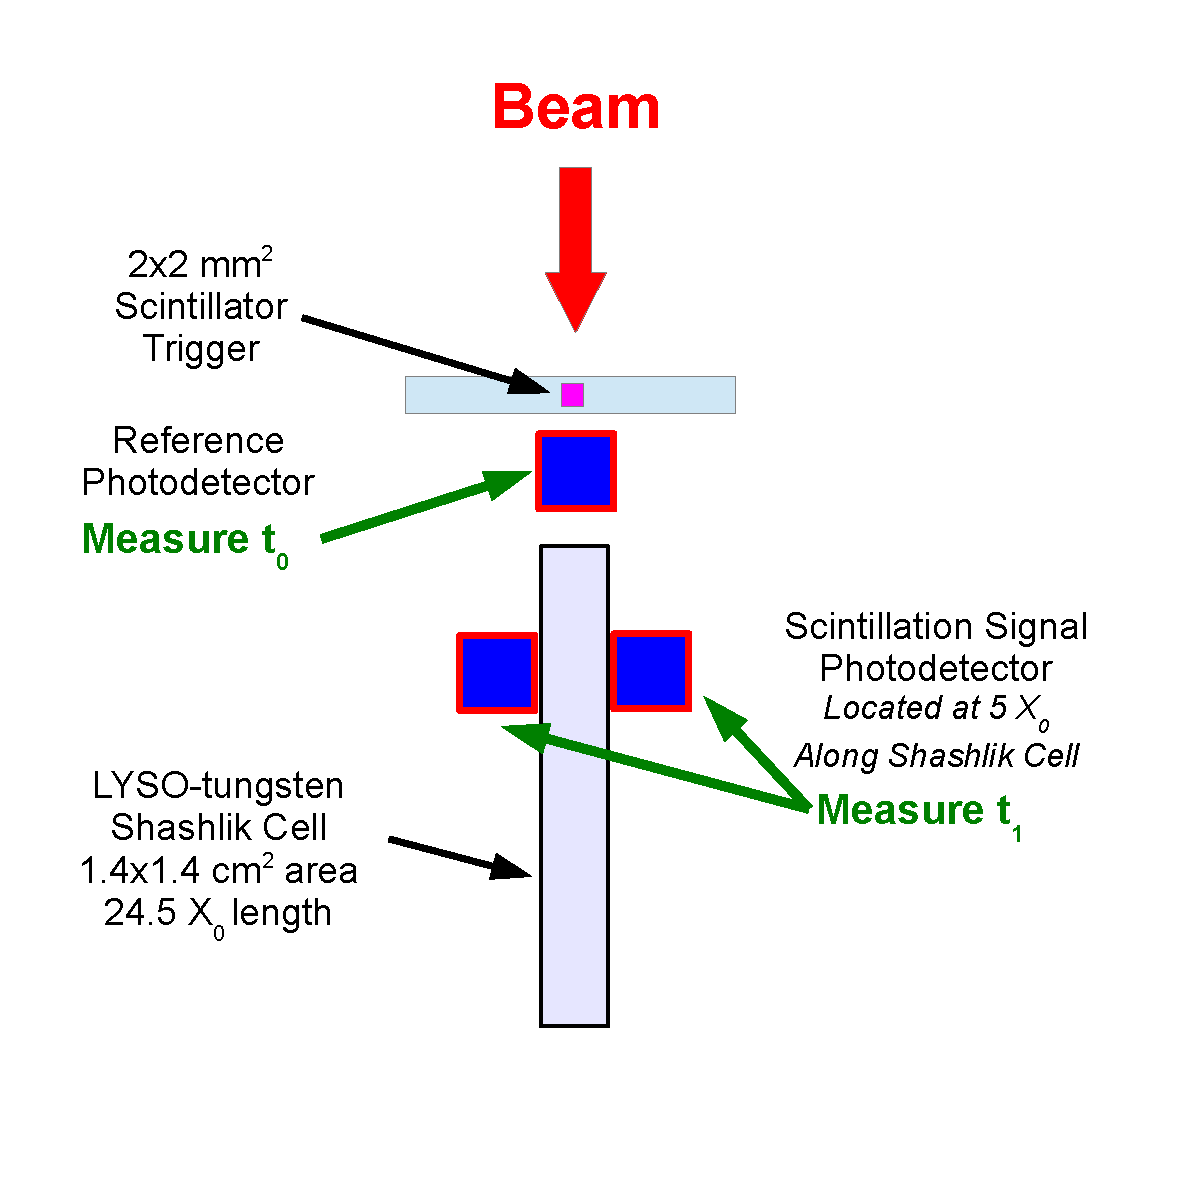
\includegraphics[width=0.45\textwidth]{figs/ShashlikSideReadoutSetupSchematic} 
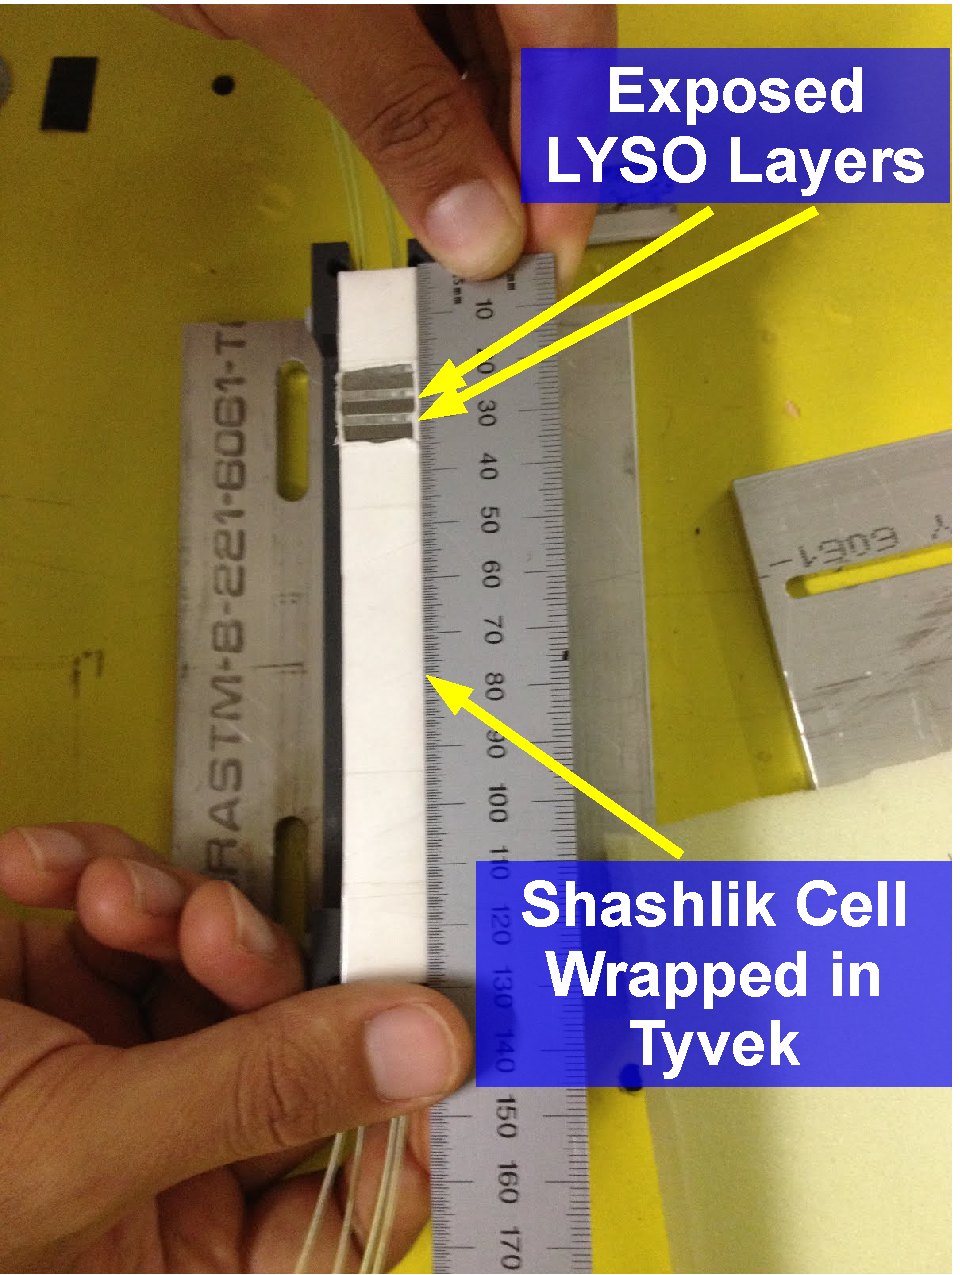
\includegraphics[width=0.45\textwidth]{figs/ShashlikSideReadoutPhotoA} 
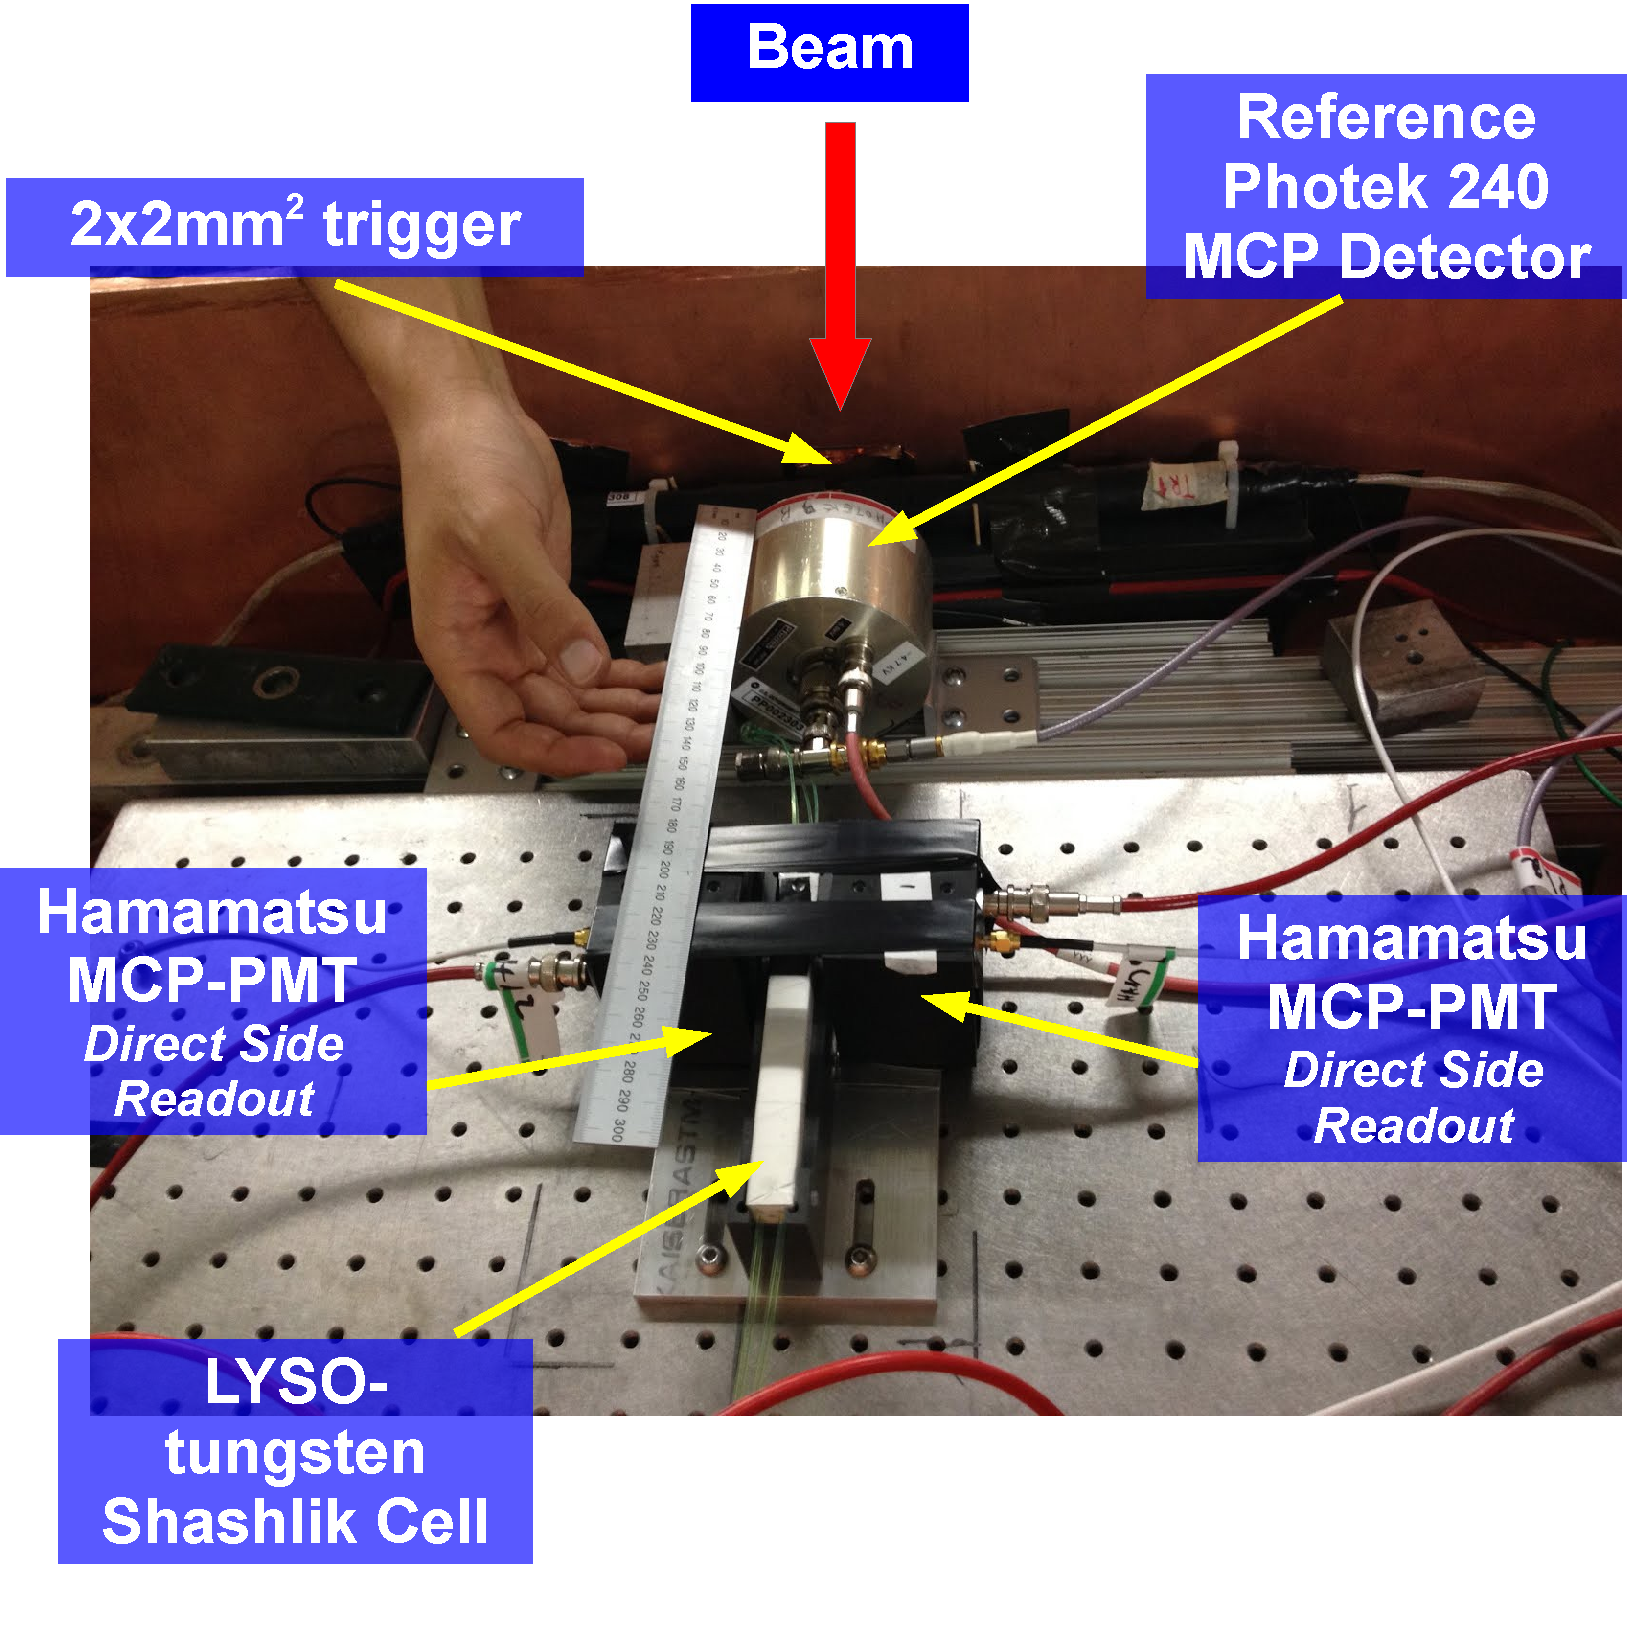
\includegraphics[width=0.45\textwidth]{figs/ShashlikSideReadoutPhotoB} 
\caption{ A schematic diagram of the experimental setup for the
time of flight measurement using the LYSO-tungsten shashlik calorimeter
with signal extraction from the edges of two LYSO layers is shown. Photographs
of the exposed edges of the LYSO layers and the full experimental setup is shown. } 
\label{fig:ShashlikSideReadoutSetup}
\end{figure}

With the intention to study the relationship between the impact of the 
optical transit time jitter and the impact of limited photostatitics,
we minimize the distance that the scintillation light
must travel to reach the photodetector in this setup and thereby minimize the
impact of optical transit on the time resolution, but reduce the photostatistics 
as we collect light from only a fraction of the edges of two LYSO layers. 
In Figure~\ref{fig:ShashlikSideReadoutTOF}, we show the 
time of flight distributions for electron beams at various energies, 
fitted to gaussian functions. The resulting
$\sigma$ parameter of the gaussian is plotted as a function of the
beam energy in Figure~\ref{fig:ShashlikSideReadoutTOFResolutionVsEnergy}.
The best time of flight resolution that we obtain is about $55$~ps, and
fitting the result to the sum of a $1/\sqrt{E}$ term and a constant term
we find a constant term of about $30$~ps with an uncertainty of $30\%$. 

\begin{figure}[h] \centering
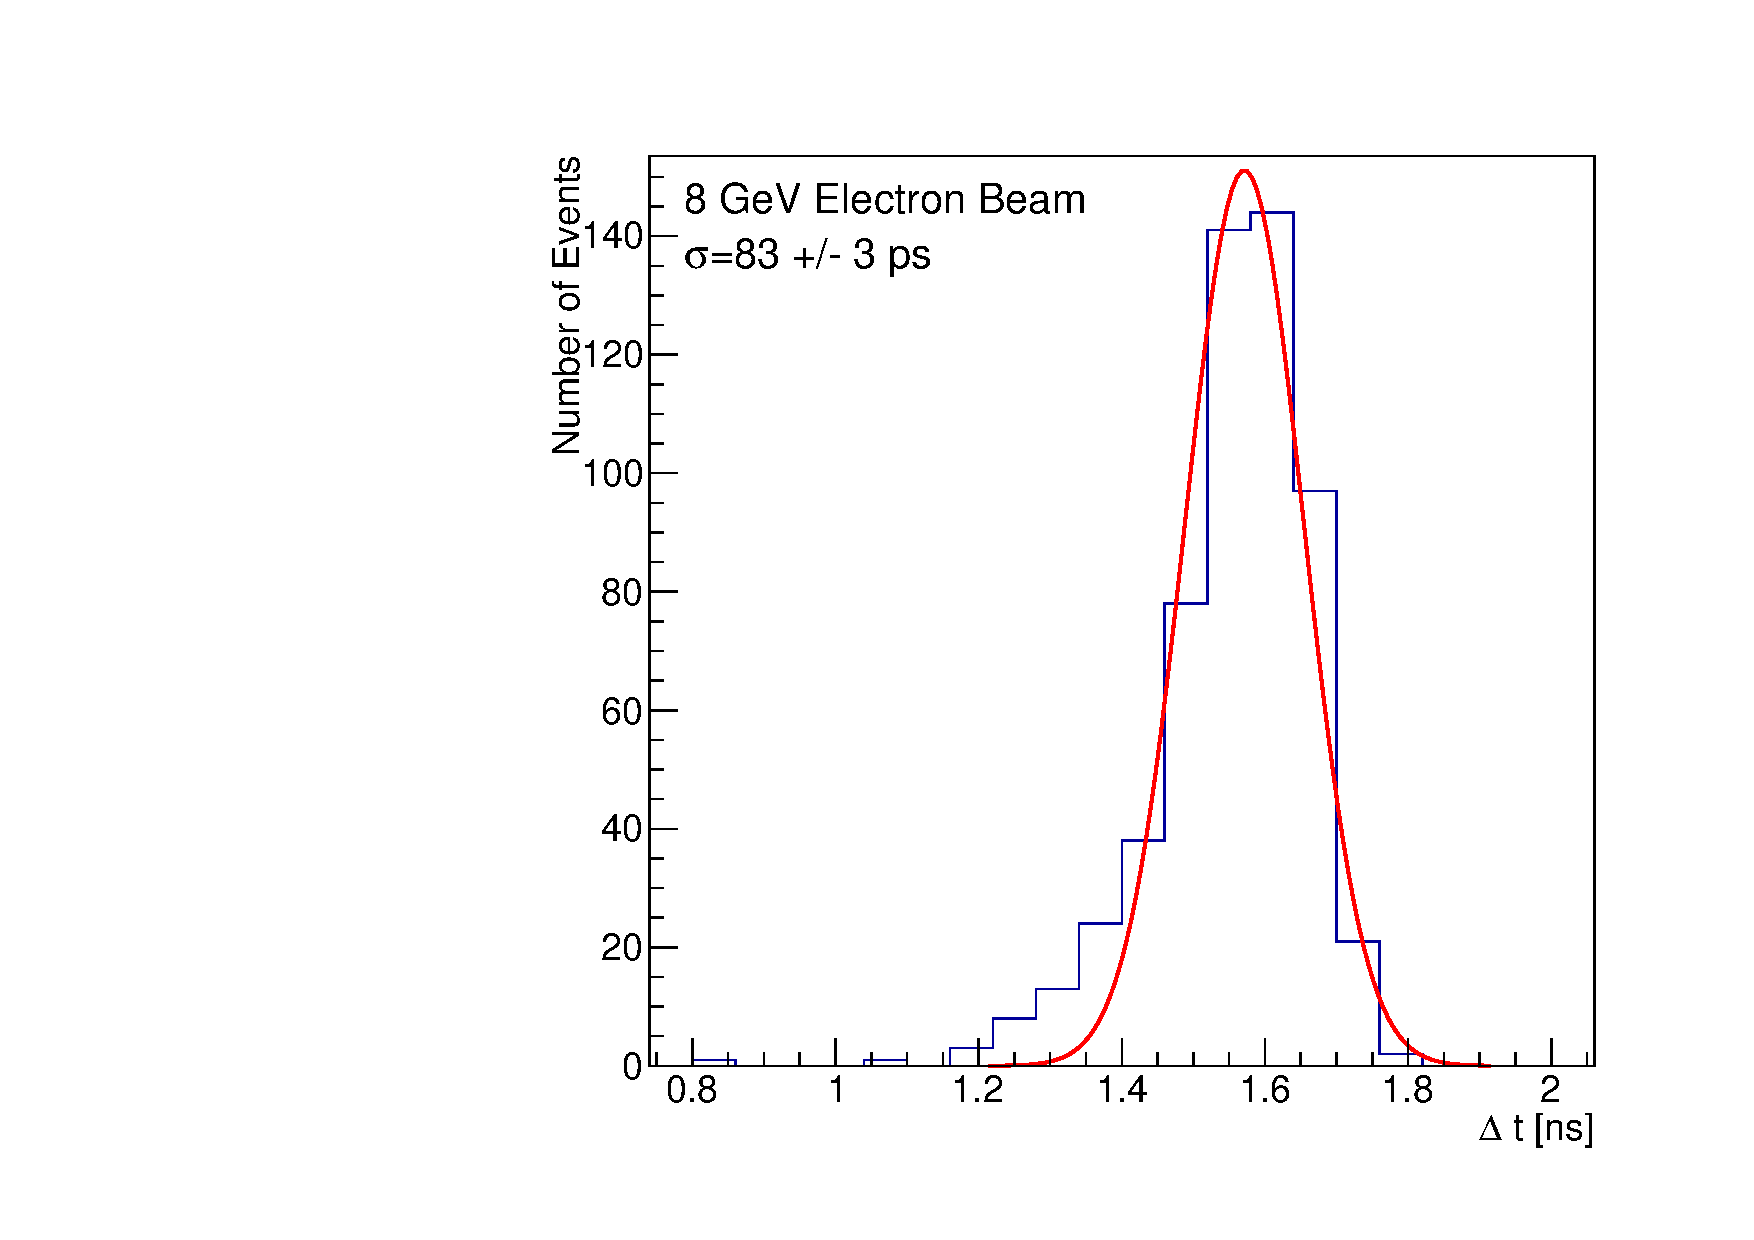
\includegraphics[width=0.45\textwidth]{figs/TOF_ShashlikSideReadout_Electron_8GeV} 
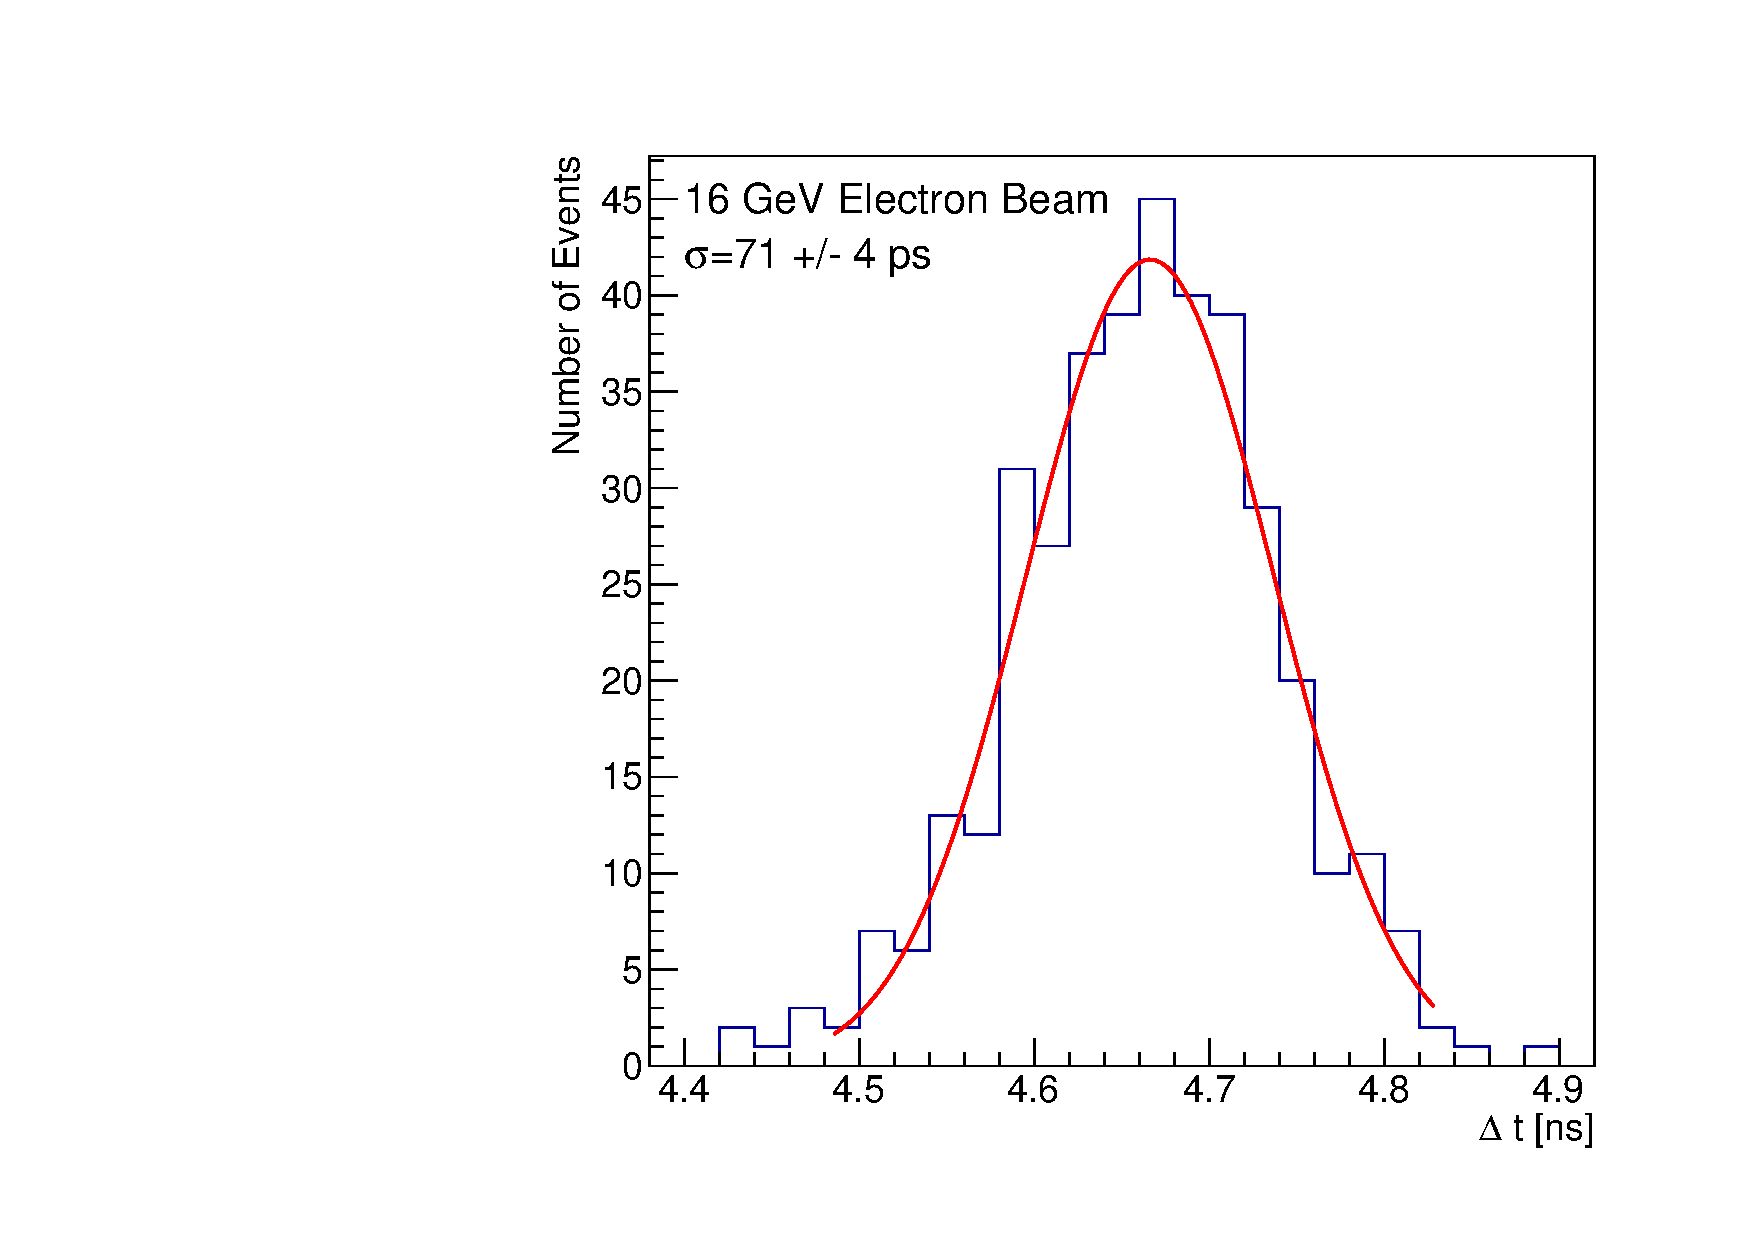
\includegraphics[width=0.45\textwidth]{figs/TOF_ShashlikSideReadout_Electron_16GeV} 
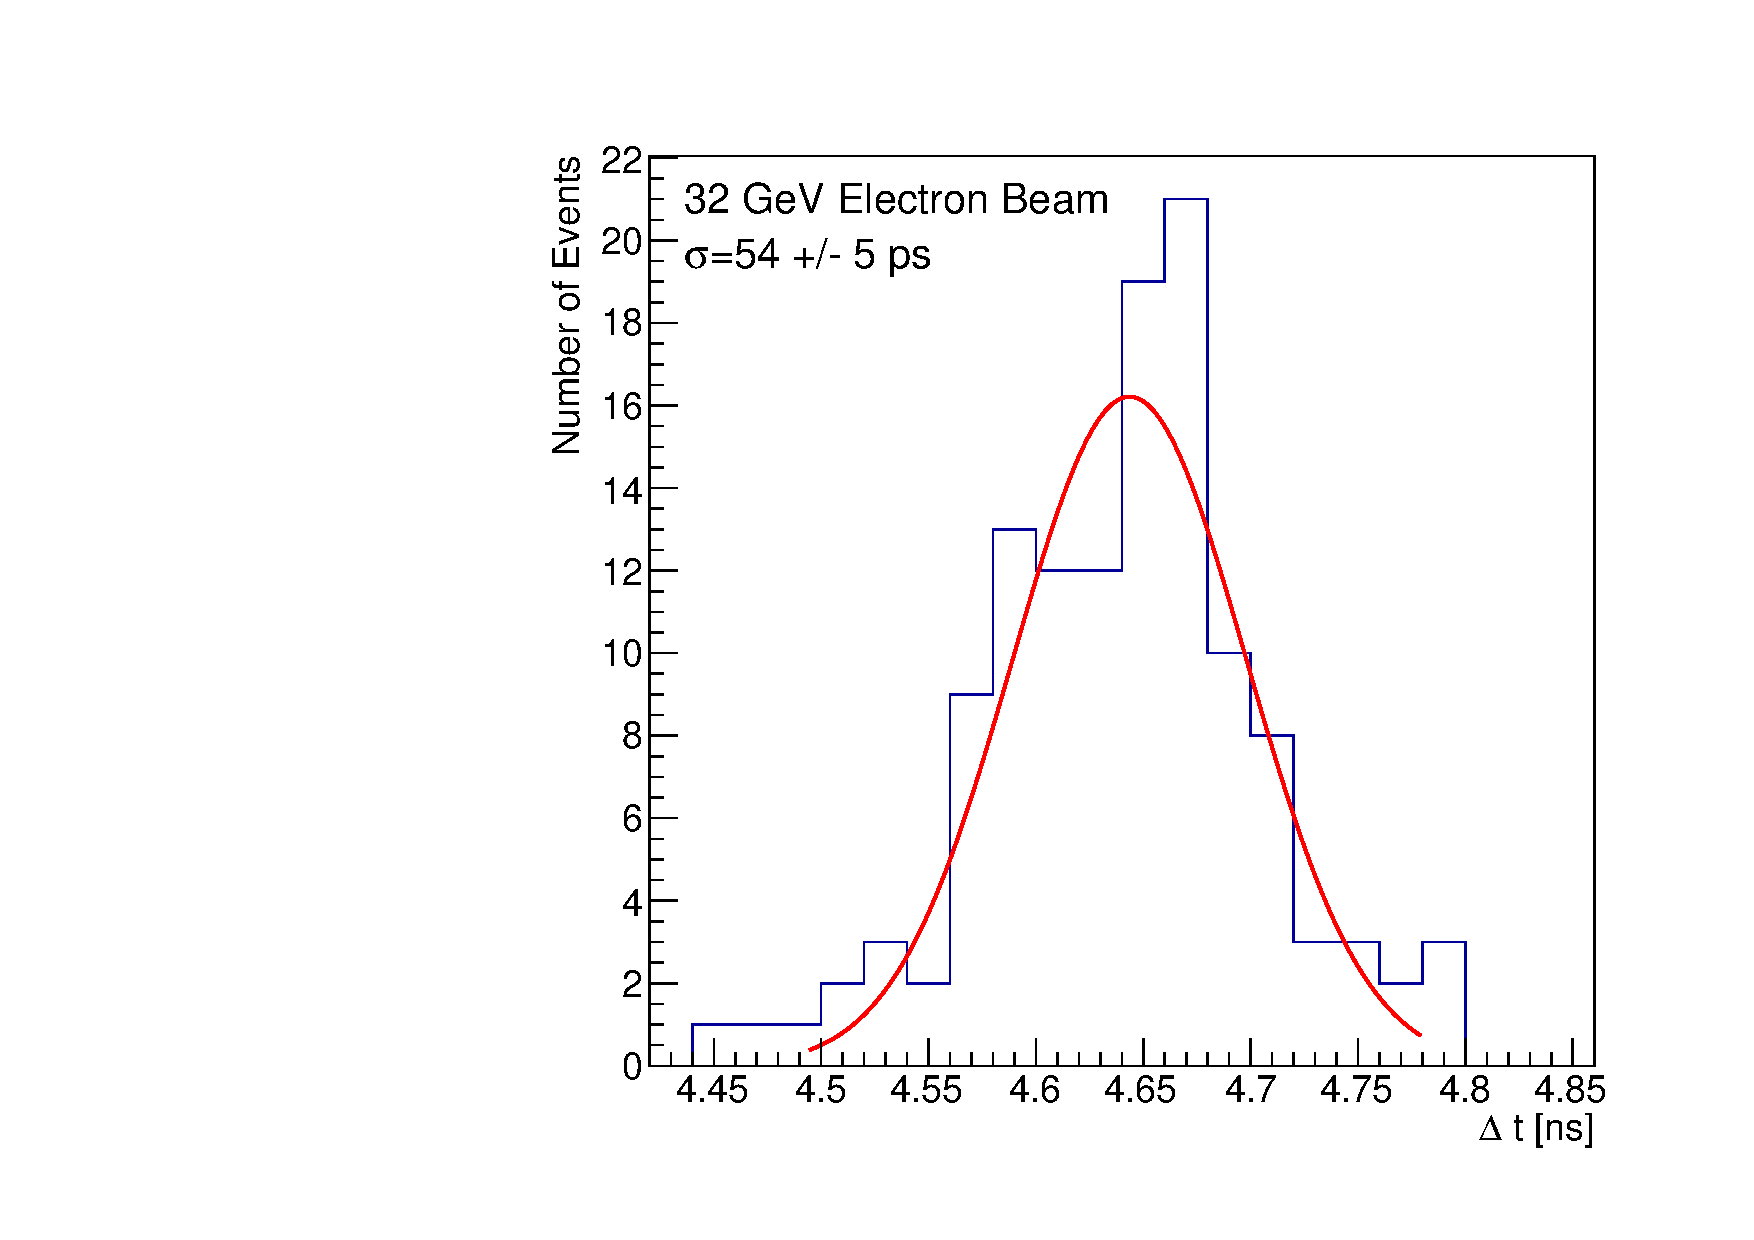
\includegraphics[width=0.45\textwidth]{figs/TOF_ShashlikSideReadout_Electron_32GeV} 
\caption{ Time of flight distributions for the LYSO-tungsten shashlik calorimeter
with signal extracted from the edges of two LYSO layers. } 
\label{fig:ShashlikSideReadoutTOF}
\end{figure}

\begin{figure}[h] \centering
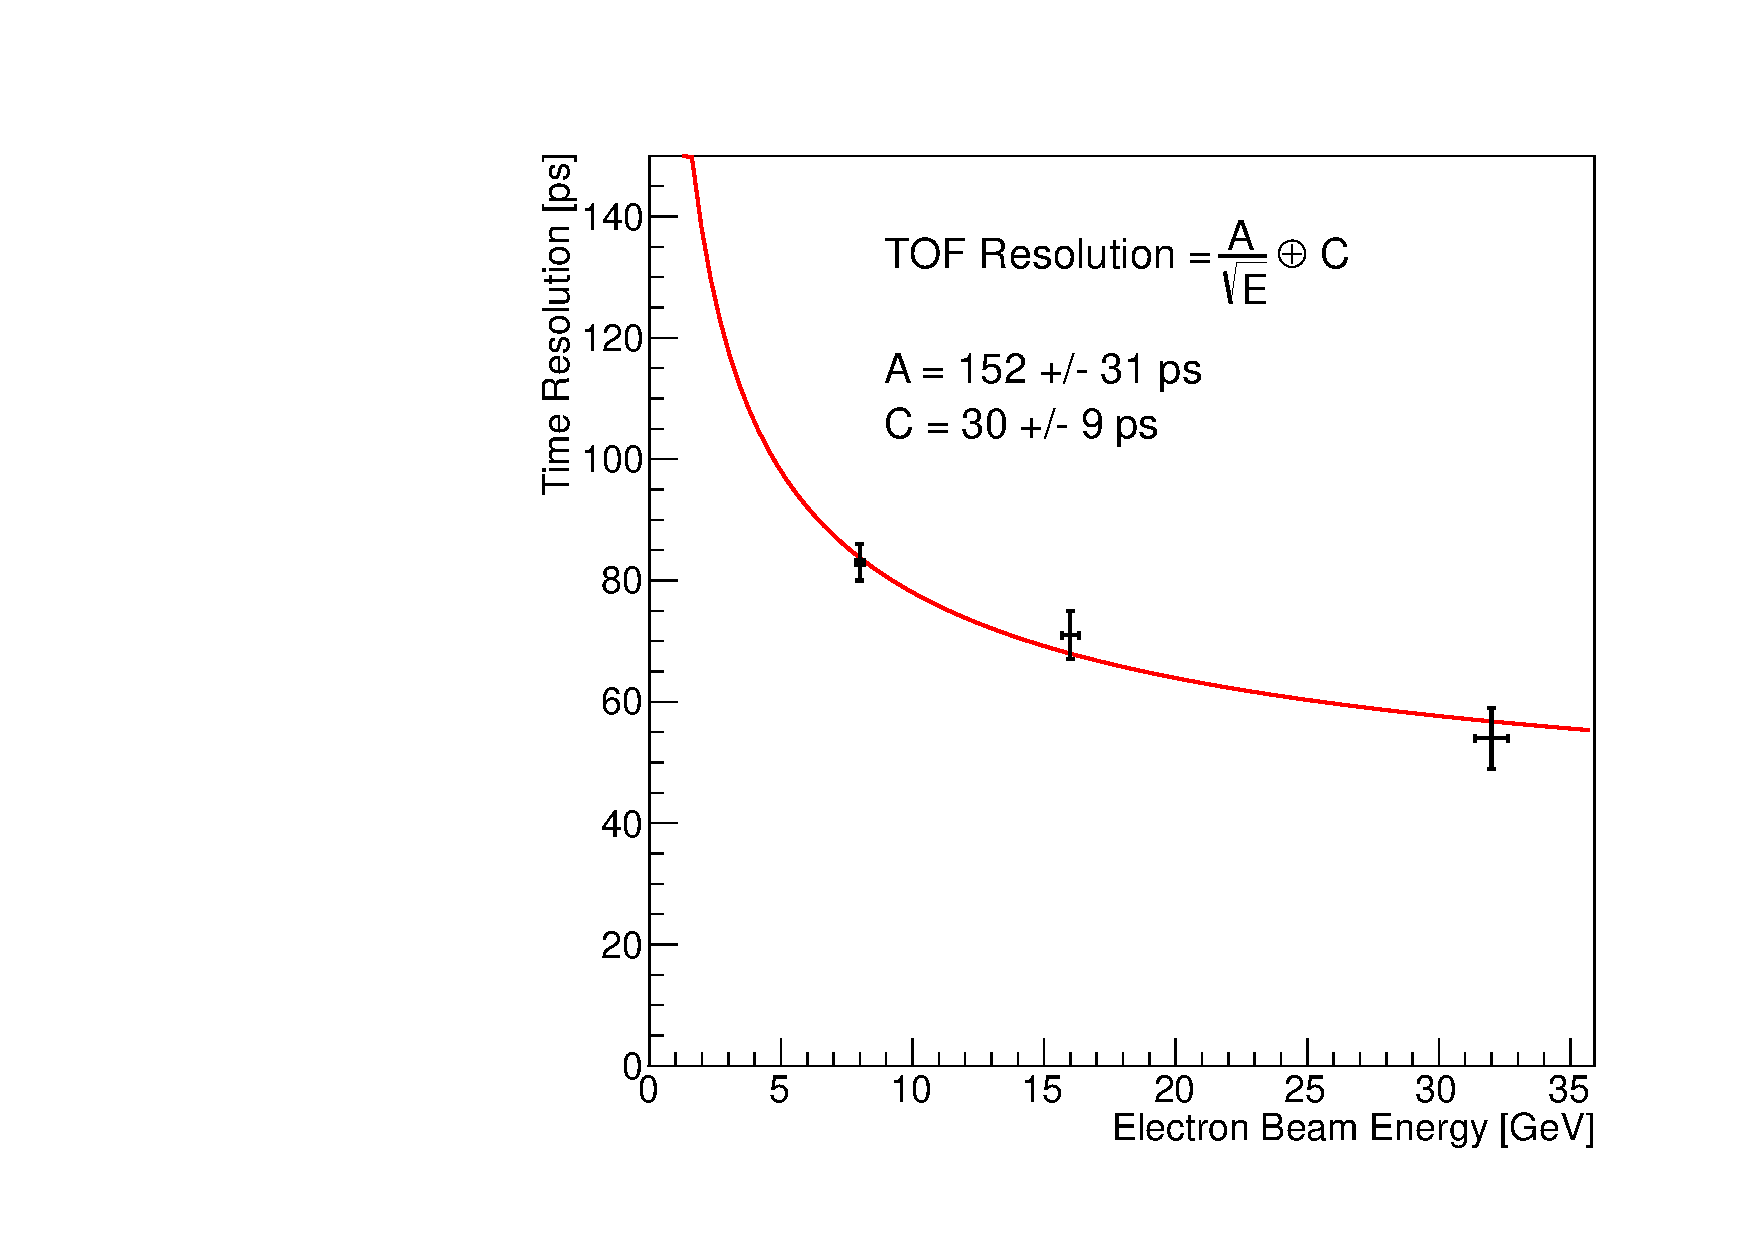
\includegraphics[width=0.45\textwidth]{figs/TimeResolutionVsEnergy_ShashlikSideReadout} 
\caption{ The time of flight resolution measured using the LYSO-tungsten shashlik calorimeter
with light signals extracted by direct optical coupling to the edges of two LYSO layers 
is plotted as a function of the electron beam energy, and fitted to the sum 
of a $1/\sqrt{E}$ term and a constant term. }
\label{fig:ShashlikSideReadoutTOFResolutionVsEnergy}
\end{figure}

In summary, we find that removing the impact of the wavelength shifting mechanism
and minimizing the impact of the optical transit does indeed improve the time
of flight resolution, but at a cost in photostatistics. Results obtained in this
experiment suggest that the LYSO-tungsten shashlik calorimeter with edge
signal readout design can likely achieve a $30$~ps resolution provided 
some improvement to light collection is achieved.

\section{Summary}

\end{document}  






























